\documentclass[a4paper, 12pt, twoside]{uiophd}
\usepackage{graphicx}
\usepackage[utf8]{inputenc}
\usepackage{multirow}
\usepackage{listings}
\usepackage{supertabular}
\usepackage{cite}
\usepackage{amsthm}
\usepackage{tikz}
\usepackage{framed}
\usepackage{pdfpages}
\usepackage[toc]{appendix}
\usepackage{pdflscape}
\newcommand*\circled[1]{\tikz[baseline=(char.base)]{
            \node[shape=circle,draw,inner sep=2pt] (char) {#1};}}

\newcommand{\jcode}[1]{\textnormal{\texttt{#1}}}
\newcommand{\pcode}[1]{\textnormal{\texttt{#1}}}
\newcommand{\pmodule}[1]{\textnormal{\texttt{#1}}}
\newcommand{\rdfterm}[1]{\textnormal{\textsf{#1}}}

\include{helpers}
\PassOptionsToPackage{hyphens}{url}\usepackage[pdftex,linktocpage]{hyperref}
\hyperbaseurl{https://github.com/}
\hypersetup{  
  pdfinfo={  
    Title={SPARQL on the Open, Decentralised Web},  
    Author={Kjetil Kjernsmo}
  }  
} 
\newtheorem{problem}{Problem}
\newtheorem{example}{Example}

\begin{document}
\title{SPARQL on the Open, Decentralised Web}
\author{Kjetil Kjernsmo}
%\institute{Department of Informatics,
%Postboks 1080 Blindern,
%0316 Oslo, Norway}

%\email{kjekje@ifi.uio.no}

\frontmatter
\maketitle
\newpage
This page was intentionally left blank
\newpage

\begin{abstract}
  This dissertation discusses a broad range of problems concerning the
  use of the SPARQL query language on the open, public Web. It is
  motivated from seeing decentralisation of data and infrastructure as
  an important social goal, and SPARQL as an enabling technology to
  solve problems using the Semantic Web. The dissertation makes
  contributions in hypermedia, where RDF is used to create a format
  that can tell humans and machines alike how to manipulate resources
  on the Web; philosophy of science, where important foundational
  problems around how to create valid knowledge and objectivity are
  discussed; statistical methods that better satisfies the
  requirements from philosophy of science than current practice; how
  to improve developer efficiency with novel programming paradigms;
  and finally how caching infrastructure in the Internet may be used
  to make query answering across the Web more robust.

\end{abstract}

\section*{Acknowledgements}

First and foremost it is my pleasure to thank my caring wife Hege,
whose invaluable support and affection has been critical to carry
through this project, and then my children Synne, Eivind and Marius,
two of whom have been born while working on this, for putting up with
a father that sometimes has his mind in the computer. My deceased
parents Ragnhild and Dag has had a major impact with their stimulus
throughout childhood and their enduring support. Arguably, allowing me
to use the 1985 PC with no graphics adapter to write programs was the
start of this project.

My advisers Martin Giese and Arild Waaler deserves a big thanks for
kickstarting the project, help adjusting its course over the years and
thorough and enlightened criticism of manuscripts prior to submission.

I would like to thank my co-authors: In particular Gregory Todd
Williams, who have not only co-authored a paper, but written much of
the underlying software I use, formed the standards that this work
builds on, and been a great discussion partner and friend. John
S. Tyssedal deserves a big thanks for agreeing to write a paper where
we started out with very little common ground. Discussions with Ruben
Verborgh always creates the right amount sparks to be enlightening,
and it has been a pleasure to become friends.

It is also a pleasure to thank the entire Semantic Web community for
their openness and welcoming attitude. Whether you come as a hacker
or want to pursue standardisation, you are likely to meet people like
Dan Brickley, Charles Nevile, Andy Seaborne, Steve Harris, Phil Archer
or Ivan Herman, all of whom have been important for my understanding
of the Semantic Web. The academic community, with their important ISWC
and ESWC conferences are equally welcoming, and has culture of sharing
insight that many other academic communities would envy. Many thanks
are due to Oscar Corcho for first integrating me into the community,
Maria-Esther Vidal and Jacco van Ossenbruggen for encouraging me to
further pursue the speculations around the role of empirical methods,
and general support. Jürgen Umbrich and Axel Polleres deserves a big
thanks for welcoming me in Vienna and many discussions.

I have made many friends in the community, for which I am thankful. Of
these, the following in no particular order have in one way or the
other shaped this work through personal contact beyond published
papers: Olaf Görlitz, Norman Gray, Ansgar Scherp, Frank Van Harmelen,
Olaf Hartig, Javier David Fernández García, Aidan Hogan, Maribel
Acosta and Philip Stutz.

The Perl community have also been important in developing the ideas
and the code of this thesis. In addition to Gregory Todd Williams, I
would like to thank Toby Inkster, Patrick Hochstenbach, Chris Prather,
Kip Hampton, Robin Berjon, Shawn M.  Moore, Michael Nachbaur and Jonas
Smedegaard.

My industry colleagues David Norheim and Robert Engels have
also been important in shaping my technical understanding and my
ideas.

Finally, many thanks to Helen Murray for linguistic assistance.


\tableofcontents
\mainmatter

\chapter{Introduction}

\section{Semantic Web Technology}\label{sec:semwebtech}

The World Wide Web, or just the Web for short, is a well-known global
information space invented by Tim Berners-Lee in 1989, that further emerged
in the 1990s. It is characterised first and foremost by its
universality, anyone can set up a computer, connect it to the Internet and
start serving data or documents from it, and further adapt it to their purpose. 

The Semantic Web is an extension of the Web that has been under
development since 1997\footnote{The first working group draft of the
  RDF specification is dated 1997-08-01, see
  \url{http://www.w3.org/TR/WD-rdf-syntax-971002/}.}, to extend the
Web with languages for expressing information in a machine processable
form\cite{semwebroadmap}.

\subsection{Basic technology}

The Semantic Web is built on a number of specifications that has been
developed under the auspices of the World Wide Web Consortium. The
core technology is known as the Resource Description Framework
(RDF). The framework is defined in a suite of specifications, defining
concepts and abstract syntax, semantics, and several concrete
syntaxes.

Conceptually, an RDF statement is a triple, where the terms are a
subject, a predicate and an object. The building blocks for these
triples are literals, blank nodes and Internationalized Resource
Identifiers (IRI). IRIs builds on the familiar URL: Uniform Resource
Locator, informally known as a Web address,
e.g. \url{https://www.w3.org/RDF/} is an address for a document about
RDF. It is also the document that lists the specifications that the
following outline relies. 
On the Semantic Web, the URL is first generalised to a Uniform
Resource Identifier, URI, that can not only name a document on the
Web, but any resource. A resource can be a physical thing, like a
person, or an abstract thing, like the type of weather at some place
at some time, numbers, strings, etc. Then, URIs are extended to IRIs
to enable the use of any character in them. Literals are strings with
a datatype (denoted by a IRI), and optionally a language tag. Finally,
blank nodes are unnamed nodes. RDF defines which of these building
blocks may be used for what term: The subject may be a IRI or a blank
node, the predicate only a IRI, whereas the object may be a literal,
blank node or IRI.

The use of IRIs makes it possible to view RDF statements as a directed
graph, where the subject IRI is a vertex, the predicate is an edge to
an object vertex\footnote{A working draft of the RDF Semantics
  specification dated 23 January 2003, see
  \url{https://www.w3.org/TR/2003/WD-rdf-mt-20030123/}, described the
  graph structure as a partially labeled directed pseudograph with
  unique node labels.}.

For historical reasons, the first syntax that was standardised for RDF
was an syntax based on the tree-structured Extensible Markup Language
(XML). The simplest standardised syntax is known as N-Triples, where
each statement is written on a single line, where each IRI is written
out in full. The basic building blocks of N-Triples has been reused to
create a compact and natural text form syntax, known as Turtle. Turtle
has gained traction, and is well established as a common syntax. A
simple graph expressed in Turtle could be:

\begin{example}{Turtle syntax}\label{ex:turtle}
\small
\begin{verbatim}
@prefix foaf: <http://xmlns.com/foaf/0.1/>.
@prefix dct:  <http://purl.org/dc/terms/>.

<http://www.kjetil.kjernsmo.net/foaf#me> a foaf:Person ;
  foaf:name "Kjetil Kjernsmo" ;
  foaf:made <http://folk.uio.no/kjekje/2013/iswc.pdf> .
<http://folk.uio.no/kjekje/2013/iswc.pdf> a foaf:Document ;
  dct:title "Introducing Statistical Design of [...]" ; 
  dct:creator <http://www.kjetil.kjernsmo.net/foaf#me>, 
              <http://[...]/person/john-s-tyssedal> .
\end{verbatim}
\normalsize
\end{example}

The example opens with prefix declarations, to allow abbreviating
IRIs, e.g. the predicate \rdfterm{foaf:name} is an abbreviation of the
IRI \rdfterm{\nolinkurl{http://xmlns.com/foaf/0.1/name}}. The IRI
\rdfterm{\nolinkurl{http://www.kjetil.kjernsmo.net/foaf\#me}} is a name for this
author. The \rdfterm{a} predicate is standards-defined abbreviation
for \rdfterm{\nolinkurl{http://www.w3.org/1999/02/22-rdf-syntax-ns\#type}}, which
is used for declaring the subject an instance of a class, in this case
\rdfterm{foaf:Person}. Then, the \rdfterm{foaf:made} predicate
is used to link to an author-published version of one of the
publications of this dissertation, and further information is then
provided about this publication, including a link to the co-author. As
we see, semicolons are used to separate statements that share a
subject, commas separate statements with the same subject and
predicate, while periods terminate a statement. \texttt{[...]} is just
to shorten the lines in the example and is not a part of the syntax.

Note that all the IRIs uses the HTTP scheme. The Hypertext Transfer
Protocol (HTTP) is the main application protocol used on the Internet
for the Web, and is also the protocol used most for the Semantic
Web. It is a request-response protocol in a client-server computing
model, but also accommodates for intermediate proxies. HTTP messages
consist of a header, typically with metadata, and a body, which is the
content itself. The standard defines several headers that can be used
to control caching on either the client, the server or an intermediate
proxy.

Also, note that all IRIs in this example are \emph{dereferenceable},
meaning that if an HTTP client is used, a representation of the
resource can be retrieved across the Internet. This, along with that
it is expressed as RDF, makes the above so-called Linked Data.

HTTP IRIs are not the only possible choice, to the contrary, the
scheme and what may be associated with it, such as a protocol, is an
orthogonal issue to the data model and syntax, and any IRI scheme can
be used.

\subsection{Interacting With Data}\label{sec:introinteract}

To read and write this graph, several techniques have been
developed. For reading, one is to simply parse the string into a
suited data structure and use any tool available in the chosen
programming language to examine the data structure, or simply write
data to e.g. a Turtle string.

A more sophisticated approach is to match parts of the graphs using
\emph{triple patterns}. A triple pattern may contain variables for
certain terms, for example:

\begin{example}{A triple pattern}
\begin{verbatim}
?subject a ?class .
\end{verbatim}
\end{example}
This triple pattern will match the two triples 
\begin{example}{Triples matched by triple pattern}
\small
\begin{verbatim}
<http://www.kjetil.kjernsmo.net/foaf#me> a foaf:Person .
<http://folk.uio.no/kjekje/2013/iswc.pdf> a foaf:Document .
\end{verbatim}
\normalsize
\end{example}
from the above example (prefixes omitted for brevity). Frameworks in
popular programming languages commonly have a method that implements
this.

The triple pattern is also a fundamental building block of the SPARQL
query language, which is the language that is the main topic of this
dissertation. SPARQL is an extensive, standardised query language with
both read and write operations. The syntax is near Turtle, but as the
above triple patterns, introduces variables. A set of triple patterns
may be used to create a conjunctive query, and along with a filter
that can be used to further constrain the query with boolean
expressions. Together, they are known as a Basic Graph Pattern
(BGP). More advanced parts of the language are built around BGPs.

SPARQL also introduced a mechanism for naming a graph or parts of a
graph with a IRI, an approach that was subsequently adopted by
RDF. Therefore, RDF is today often implemented not just a expressed as
a triple, but may be a expressed with a quad.

To execute a query, a SPARQL engine would typically parse the query to
create a tree of algebra objects (in the case where an object oriented
programming language is used) in the process. Then, a query planner
component would traverse the algebra tree, and for each algebra object
or branch of algebra objects, the query planner finds various ways to
access the data in the underlying store or execute other
operations. In many programming frameworks, the only way to access
data is through matching a triple pattern. If that is the case and
the incoming query consists of just a BGP, the query planner's task
would simply be to match all the triple patterns and join their
results, and finally apply any constraining filters. 

However, even though the result does not depend on the order of
execution of a BGP, the time it takes to find the result often does. For
example, consider the following BGP:
\begin{example}{A Basic Graph Pattern}\label{ex:bgp}
\begin{verbatim}
?subject foaf:name ?name ;
         foaf:workplaceHomepage <http://example.com/> ;
         foaf:made ?contribution .
\end{verbatim}
\end{example}
In most cases, if the triple pattern with the \rdfterm{foaf:name}
predicate is evaluated first, it is likely to match many resources,
since nearly everything may have a name, and therefore, it does not
reduce the number of statements that needs to be searched when
matching the next triple pattern by much. Instead, the
\rdfterm{foaf:workplaceHomepage} may be matched first, as we may guess
the fact that the object is given will be more restrictive, but that
too fails if everyone in the database works for the same organisation
and has used this predicate. It is the query planner's task to choose
between equivalent plans to ensure that the most efficient evaluation
is chosen. As is clear from this example, it is often insufficient to
rely on such heuristics, and therefore, it is common to rely on a
statistical digest in the query planner. Still, the task of query
planning remains a very complex one, and often, insufficient
statistics is available, so that planning is done using heuristics or
based on assumptions that do not hold. These are only some of the
concerns that affect performance of the overall query engine.

Indeed, detailed knowledge of the data, such as a comprehensive
statistical digest may be available close to the database, but is not
exposed in ways that higher levels in the technology stack can make
use of. In our case, this is especially true for a caching proxy.

\subsection{Hypermedia}

However, in terms of utility when programming, advanced query
languages such as SPARQL may not be needed for many applications, and
may represent an overly high barrier to entry.

Hypermedia is the idea that all information needed to drive
interaction in an application must be readily available in the
request-response dialogue. For human interactions, this has been
understood as a requirement for a long time, one has to tell the user
how to interact with the application, if not, the user is unlikely to
be able to solve the task. Contemporary efforts now extend this to
machine-machine interactions. 

In this context, hypermedia types is a way to classify what kind of
operations a certain media type can help the application perform.

\section{Contributions}\label{sec:contribsum}

The present work is located at the confluence of several contemporary
efforts in the Semantic Web community. The focus is on query answering
with the SPARQL query language, with emphasis on exploiting the World
Wide Web, but it touches upon query federation, hypermedia, empiricial
methods for evaluating performance, standards compliance and even
philosophy of science. 


\subsection{Hypermedia}

\begin{enumerate}
\item A thorough discussion of the implications of Hypermedia
  Types\cite{hypermediatypes} for RDF.
\item A sketch of a vocabulary for read-write RDF hypermedia.
\end{enumerate}

\subsection{Design of Experiments}

\begin{enumerate}
\item Introduction of a path for critical practice of evaluations, that makes
  use of contemporary statistical techniques, to establish a practice
  that can be used to refute assertions on performance.
\item A didactical experiment to help researchers understand the statistics.
\item The novel application of a well-established method in
  statistics, rarely used in Computer Science, to SPARQL endpoint
  evaluation.
  
\end{enumerate}

\subsection{Development problems}

\begin{enumerate}
\item A framework to enable the use of low-level optimisations in
  databases.
\item Simplification when implementing experimental features in
  SPARQL.
\item Novel programming techniques for custom query planners.
\end{enumerate}

\subsection{Survey of HTTP Caching}

\begin{enumerate}
\item An understanding of actual usage of caching headers (metadata)
  on the open Semantic Web.
\end{enumerate}

\subsection{Philosophy of Science}

\begin{enumerate}
\item A provocation to discuss epistemological questions.
\end{enumerate}

\subsection{Software}

\begin{enumerate}
\item 5 Free Software packages that have been accepted into the recent
  versions of the Debian GNU/Linux operating system.
\item Further 5 packages that already were accepted in Debian have been
  enhanced in the course of this work.
\item Contributions to the code base were accepted by another 5
  external projects.
\end{enumerate}


\section{Overview}\label{sec:introoverview}

The World Wide Web, or just the Web for short, is a well-known global
information space invented by Tim Berners-Lee in 1989, further emerged
in the 1990-ties. It is characterised first and foremost by its
openness, anyone can set up a computer, connect it to the Internet and
start serving data or documents from it. 

The Semantic Web is an extension of the Web that has been under
development since 1997\footnote{The first working group draft of the
  RDF specification is dated 1997-08-01, see
  \url{http://www.w3.org/TR/WD-rdf-syntax-971002/}.}, to extend the
Web with languages for expressing information in a machine processable
form\cite{semwebroadmap}.



The present work sits in the confluence of several contemporary
efforts in the Semantic Web community. The focus is on query answering
with the SPARQL query language, with emphasis on exploiting the World
Wide Web, but it touches upon query federation, hypermedia, empiricial
methods for evaluating performance, standards compliance and even
philosophy of science. With a scope of this breadth, the investigation
is shallow, it is hoped that some key insights will provoke further
investigation rather than being the end of any conversations.



\section{Semantic Web -- A definition?}\label{sec:nodef}

The Semantic Web can be described as a machine-readable Web of Data,
defined by a technology stack defined by the World Wide Web
Consortium. While individual technologies can be given precise,
operational definitions, the above definition is naive and can hardly
be used operationally to derive new knowledge. The Semantic Web is a
complex, human artefact that must be understood not only in technical
terms, but also in social, economic and cultural terms. First, the Web
is not only readable, but also writeable. Whether the essential parts
of a data integration problem will be solved by e.g. pervasive
ontology alignment, a linked open vocabularies approach where many
players adopt a fairly consistent set of vocabularies, or by major
players are able to force convergence towards e.g. \texttt{Schema.org}
is an example of the social, economic and cultural mechanisms that
shape the future of the Semantic Web, see
Section~\ref{sec:semproblems} for a more elaborate
discussion. Likewise, it may not be the W3C Semantic Web stack at all
that achieves success, though unlikely at this point, it may be
something in the extension of microformats\footnote{see
  \url{http://microformats.org/}}, microdata\cite{microdata}, or
something else entirely. For a thoughtful criticism of Linked Data
with a proposed alternative, see \cite{darobin1}, but again, it is
likely that social, economic and cultural factors will be as decisive
as technical. One may say that e.g. microformats cannot help achieve
the visions that may be stated for the Semantic Web, but that again
emphasises visions, not operational definitions.

One such vision is the article by Berners-Lee, Hendler and Lassila in
Scientific American 2001\cite{berners2001semantic}, but it does not attempt such an
operational definition. Neither \cite{semwebroadmap} nor \cite{berners2000weaving} contains
such definitions. However, it is clear that an essential
characteristic of the Web, and by extension, the Semantic Web, is its
\emph{universality} and therefore, any actor should be as free as
possible to adapt it to their visions and needs. A pursuit of a
definition of the term ``Semantic Web'' would require a philosophical
treatment which would be beyond the scope of this thesis, and even
with that, may not be a fruitful exercise from a technical
perspective. 

Therefore, rather than attempt a definition, understanding is rather
promoted by following the example of \cite{berners2001semantic} and
declare a vision.


\section{Objectivity of the study}

A vision has necessarily a strong personal element. This challenges
the ideals of objectivity in scientific investigations. A longer
discussion of the desirability and attainability of objectivity in
science is beyond the scope of this thesis, but objectivity can be
challenged from many different angles
\cite{sep-scientific-objectivity}.

The impact of the Web in particular and information technologies in
general, on society is great, and research projects are often funded
because of their relevance to society. With this perspective, this
research is hardly value-free. As individual researchers, we may
develop a strong relationship to the systems we create, as we have a
great intellectual investment in them. This may influence our ability
to reject a flawed hypothesis even if we should. Even though we note
in the discussion of the contributions in Section~\ref{sec:conphil}
the weaknesses of Thomas Kuhn's philosophy of science, his insistence
of understanding science as a social endeavour stands firm.

These challenges are inescapable, and therefore, it is important that
the researcher acknowledges such problems and explicitly details their
own personal motivations, visions and possible biases to let the
reader decide whether the researcher's subjective beliefs has
influenced the validity of their contribution. 

I shall attempt to do so in the following, but also note that this
influences the writing style. There are several conventions of
scientific writing that stands in opposition to the goal of letting
the reader understand the possible influence of subjective
beliefs. The frequent use of passive voice is one such convention,
that in my opinion tries to hide subjectivity rather than alleviate
its harmful effects. If the methodology used in the investigation is
flawed, it should not be obscured by writing style, the methodology
will need to be enhanced. Double blind trials in medicine are an
example of why it is important to acknowledge the investigator's
role. That is not to say that the use of passive voice is always
inappropriate, when the role of the investigator cannot be
misunderstood, it can be used just like any other language construct.

Of less importance is the use of ``we'', when it is clear that the
work has been done by a single investigator. I hold as a general
principle that the role of the investigator should never be obscured,
and therefore, such use is inappropriate. The use of pronouns should
not differ substantially in scientific writing from other writing, and
I will use them accordingly. In particular, I will use ``we'' when
more than one person has been involved, or when the reader is included
(e.g. ``We note that...'').

\section{A personal history}\label{sec:history}

As noted in the previous section, objectivity may be challenged by a
researcher's intellectual investment in a certain field of study. I
admit that I have a very large intellectual investment in the success
of the Semantic Web. This section serves two purposes: It should give
the reader a good understanding of this intellectual investment, and
enable them to assess the impact of any subjective beliefs. Secondly,
it serves to clarify \emph{my} vision, which we noted in
Section~\ref{sec:nodef} is more important than to attempt a
definition. The vision strongly influences the motivation detailed in
Section~\ref{sec:motivation}.


I created my first Web page in December 1994, and strongly appreciated
the value of the fact that I could easily contribute to the Web, and
therefore, I quickly posted anything that I had of value, for example
a collection of my best mountaineering pictures, constrained not by
the platform, but by my own time. Initially, I learnt purely by
example, i.e. using the ``View Source'' menu item when I encountered
web pages that I liked. I also had the power to mint identifiers. 

With identifiers, and the hypertext language HTML came the fact that I
could link to anyone, and anyone could link to me was highly
empowering: Discovering that people I didn't know linked to my
material was a strong, social reward. After some time, I had tens of
thousands of visitors every month.

In 1996, I started the Web pages of the Norwegian Skeptics Society
\texttt{skepsis.no}, and therefore got the control over an entire Web
server. That was another revelation, as I could actually run code, and
from that arose the need to not just learn by ``View Source'', but
start to read the specifications, notably HTML, CSS and
HTTP. Appreciating the design of these specifications took a while,
but eventually, the value of orthogonal specifications and separation
of concerns became apparent. Also, at the same time, I realised that I
could be standing on the shoulders of giants by using Free Software.

When the RDF working drafts were first published, I was first
inundated by the amount of new text to read, but at the same time I
had a growing realisation that getting information out was not solving
the problem The Norwegian Skeptics Society needed to solve: We needed
to push information into closed minds. My initial plan to address that
was to enable a higher degree of targeting of information, and a Web-wide
conversation. To do that, I wanted to create a large thesaurus of
topics of interest, and create annotations of the type ``this article
is a rebuttal of that article'', and an index that browsers could
query, so that when a user viewed an article, they would also get a
critical context. At the same time, Netscape was open-sourced as
Mozilla, and so, I was quite convinced I could contribute the code
needed for this to be accepted. 

I shared these ideas on some mailing lists in August 1998, and one of
the persons who responded was Dan Brickley, who would chair the RDF
working group. He quickly convinced me that RDF was not something to
be afraid of, quite the contrary, it was exactly what I needed.

However, all the above had happened on my spare time, as the topic of
my study was something else entirely: Cosmology, and so the interest
laid dormant for a few years as I finished my Cand. Scient.-degree. 
After that, I got some limited funding to write what today would be
called a Semantic Content Management System. The project was far too
ambitious and largely a failure, but it got me some valuable
experience with Semantic Web technology.

I was convinced that the things that made the Web great to work with
had to be present in the Semantic Web as well: Everybody is empowered
to publish, find and quickly make use of Free Software, learn by
``View Source'' (an idea which becomes even more powerful with
semantics, as if you can understand what you are viewing simply by
looking at the message, you can begin processing it), anyone can mint
identifiers, anybody can reuse those identifiers in their own
contexts, and eventually graduate to reading technical materials as
needed. Many of these things are virtues of the Semantic Web as it is
an extension of the Web, others have not been sufficiently cultivated
or even appreciated. Moreover, my experience corresponds to the
virtues that Tim Berners-Lee has attributes the Web's success
to\footnote{see
  \url{http://dig.csail.mit.edu/2007/03/01-ushouse-future-of-the-web}}.

It was not until I joined Opera Software in 2005 to work on the now
defunct Opera Community social networking site, that I had a bit more
time to work on Semantic Web technology. When I joined, they had
rudimentary support for an RDF/XML-based ``Friend of a Friend'' (FOAF)
export, which I improved before the initial release. At the time, it
was not anticipated that everything would have a URI, so Dan Brickley
was a proponent of the view that most things, including people, would
be identified mainly by their properties, e.g. their email address. It
was a certain tension between that view and the ``give everything a
URI''-movement heralded by Tim Berners-Lee at the time, but I decided
to place myself in between, by giving everything a URI, but at the
same time ensure that enough properties would identify people. I also
included outward links, so that people could integrate the database
export we provided with their hand-maintained FOAF. I also added
support for photo gallery metadata and linking tags as given in a
personal SKOS-ontology to Wordnet to enable assigning clearer meaning
to tags. This effort was acknowledged in the Linked Data Design
Issue\cite{linkeddataissue} that formed the basis for the more recent Linking
Open Data project.

However, at this point, I started to realise that it was difficult to
develop applications around traversing Linked Data, and that
prompted me to consider the possibility to offer the ability to
execute arbitrary queries. On 2005-11-30, I published the first public
SPARQL endpoint with actual production data\footnote{see
  \url{http://www.onlamp.com/pub/wlg/8609}}, consisting of 2695114
triples, but it quickly grew to \~15~million triples.

Unfortunately, it wasn't allotted time to enhance and document the
SPARQL Endpoint further, and it didn't see much practical use. 
I was, however, allowed to join several World Wide Web Consortium
groups. First, the Web Content Label Incubator Group, which was tasked
with discussing a replacement for the then archaic Platform for
Internet Content Selection, and resolved to use RDF for this
purpose, and it transitioned into the POWDER Working Group, which
provided the specifications. 

More importantly, I joined the Semantic Web Education and Outreach
(SWEO) Interest Group, where I admitted my frustration with the lack
of practical progress with Semantic Web technologies and the relative
lack of uptake. This sentiment was echoed by the late Aaron Swartz,
who was asked by the group on his opinion, and he emailed the
following statement\footnote{see
  \url{https://lists.w3.org/Archives/Public/public-sweo-ig/2006Dec/0138.html}}:
\begin{quote}
I'm not sure what SWEO is, but my feeling is and pretty much always
has been that the Semantic Web people need to start putting together
Genuinely Useful stuff that can be done Right Now.
\end{quote}

This was one of the motivations I had for starting the SWEO Community
Projects, where a questionnaire was posted on the Web, and people from
the Semantic Web community were challenged to come up with a project
that would provide practical benefits in the short term. We received
10 proposals, out of which 3 was selected for backing by the SWEO
IG. None of them were successful, but a fourth proposal, submitted by
Chris Bizer and Richard Cyganiak built momentum quickly and was
therefore also selected for backing, despite some criticism by several
IG members, myself included. The proposal was titled ``Linking Open
Data'' and sought to take already abundant open data and model it
using guidelines of the Linked Data Design
Issue\cite{linkeddataissue}. LODstats\cite{auer2012lodstats} provides
extensive statistics on the results of this project, and has of this
writing seen nearly 10~000 data sets.

At this point, I left Opera to work as a consultant on Semantic Web
technologies. One of the projects that were successfully completed was
called Sublima\cite{sublima}. It was driven entirely by RDF and SPARQL,
and featured faceted navigation, navigation in a thesaurus, and full
text search. Experiences from this project influenced requirements of
SPARQL 1.1 \cite{sparql11query}, and I was an editor of the SPARQL 1.1 Features and
Rationale specification\cite{sparql11new}. Parts of the property paths
feature and aggregate queries were used extensively. Write operations
were also implemented with SPARQL using what was then specified only
in a member submission to the W3C\cite{seaborne2008sparql}. This was the basis for
the update language in SPARQL 1.1 but differed substantially in
surface syntax, partly because our work showed how certain usage patterns
could be simplified. 

Two features that arose from Sublima requirements were not accepted
for SPARQL 1.1, however: Full text index and a feature known as
``Limit Per Resource''\footnote{see
  \url{http://www.w3.org/2009/sparql/wiki/Feature:LimitPerResource}}. The
latter feature arises from the fact that usually, the user is
indifferent to the number of solutions to a query, and therefore
limiting by the number of solutions is unhelpful. This is especially
true since other features of SPARQL, such as optional clauses, are
helpful in dealing with heterogeneous data. In the Sublima case, it
was interesting to limit by the number of articles that were returned,
but the number of solutions depended on the number of authors of an
article and the concepts used to classify an article. To achieve the
desired effect with SPARQL 1.1, one would have to write a very complex
subquery, which is undesirable for such an important feature.


Another project, based on much of the same code
base replaced the SKOS ontology of the Sublima project with an OWL
ontology, and also used reasoning to aid navigation in multimedia
libraries.



However, it became clear that I could not have sufficient time in the
industry to pursue what was developing as my main interest, query
answering over data on the open Web, for generic application
development. 

While the motivation and the problem statements of this work
undoubtedly have been influenced by my intellectual investment in the
Semantic Web, the papers should show that the investigation has not.


\section{Motivation}\label{sec:motivation}

The following section provides an overview of the motivation behind
this work in general and each direction in particular. Detailed
problem statements are given in Section~\ref{sec:problems}.

\subsection{Cruise altitude view}

There is a class of diverse, yet structurally similar, problems people
face nearly every day: When we book a flight, we may be interested in
a romantic getaway, yet we are forced to select the airport of
destination first. We often end up buying the same groceries because
we don't know what will taste well together. Last time I bought a car,
the two most important features was that it had 4 wheel drive and that
the trunk was long enough to fit a full-size baby stroller
length-wise. To find a property to build a home, I took into account
the sun conditions, that it was close to public transport that would
transport me to campus within a certain time frame, close to
ski tracks, low concentration of uranium in the ground, number of children for
my children to play with, and an affordable price level. And once the
house was being built, I had to choose the toilet seat depending on
the frame in the wall and even a toilet seat that would fit.

Of fundamental importance is that even though each of these
problems are rarely encountered, there are so many such problems that
we encounter them frequently. I would like to see a Semantic Web
where the plumber delivers his offer in a manner so that the open
options can be distinguished from the constraints, where a query can
be formulated to find the area I'd like to build my house based on
such extensive criteria, where the very rare comparison between a
collapsed baby stroller and car trunk can be done, where I will be
able to cook better food without being a chef and where I can book my
travel based on what I want to experience rather than make me choose a
destination based on lacking information.

Now, all this information exists on the Web, or at the very least, in
some database, and for the most part, the above problems can be
solved by surfing many websites. We are, however, reminded of ``Connolly's
Lament'' (due to Dan Connolly, one of the Semantic Web's early champions):
\begin{quote}
 The bane of my existence is doing things I know the computer could do
 for me.
\end{quote}

Moreover, the problem could be solved by writing programs to integrate
the variety of data sources for each scenario, but this is clearly not
sustainable, as each particular integration is of interest to very
few, but the cost of the integration increases for every integration
task. Fewer people to pay for a more expensive task quickly becomes
economically infeasible.

Technically, it might be an easier problem to solve if the data could
be centralized, and that solution has been argued for by
\cite{DBLP:conf/semweb/BetzGHS12}. Nevertheless, even if all their
arguments remain valid from a technical viewpoint, the most important
arguments against centralisation are social: If important components
of the Semantic Web are under the control of some central authority, it
is likely that one cannot publish anything, link to anything, or
develop any application without permission. It may create an unhealthy
power structure, which may create commercial or intellectual
hegemonies. Tim Berners-Lee discussed this in \cite{berners2000weaving} and an
interview in Wired Magazine in 2014\footnote{see
  \url{http://www.wired.co.uk/news/archive/2014-02/06/tim-berners-lee-reclaim-the-web}}.
This is the key motivation to still design a distributed Semantic Web,
regardless of the technical difficulties that may arise.

The Crosscloud\footnote{See \url{http://crosscloud.org/}, quote
  retrieved on 2016-05-30.} project is motivated from the same
observation:
\begin{quote}
Today, in a world of cloud-hosted software, every application is a
kind of trap. Even if it lets you export your data in a form other
systems can read, many of the best apps have social features. You
can't switch because your friends or colleagues are still using the
old site — the new site will be a ghost town. This stifles competion,
blocks innovation, and leaves users less happy with the systems they
are using. While some developers might want to lock-in users, we trust
that many value user happiness and would open their systems if it was
technologically practical. Our goal is to make it practical.
\end{quote}

The naive enthusiast may now forward the claim that Linked Data is the
solution and the whole solution, and at times of hubris, I may myself
have been guilty of conjecturing that sitting down to write the code
based on what we already know would solve the problem.

At times of doubt, the large number of unsolved problems, theoretical
as well as practical become apparent. In the following, I will try to
enumarate the problems I have foreseen, discuss their place in current
research, and what problems I have attempted to tackle in this
dissertation.

Both the idea of a decentralised Web and the idea that SPARQL
endpoints can be made openly available for any query on the Internet
seems to go against the conventional wisdom of the database
community. We are, however, motivated to solve this problem by the
social requirement of decentralisation and by the use cases mentioned
at the start of this section.

It is also important to frame the question correctly: We want to
answer queries, we do not require that any remote server accepts the
entire burden of evaluating queries. It is becoming quite clear that
the current practice of evaluating any arbitrary SPARQL query on a
remote server is economically unsustainable, and it is made clear by
the instability of SPARQL endpoints on the Web \cite{buil2013sparql}.

However, we note that the Internet infrastructure is accommodating for
solving parts of this problem with the presence of caches at several
different levels. Some clients also have significant processing
capacity, and these are among the factors that could make SPARQL query
answering on the open Web practically feasible. The focus of this work
is to ease the burden of servers by allowing other parties to take
parts of the query evaluation.

\subsection{Hypermedia}

The hypermedia idea is attractive as it is the extension of the ``View
Source'' idea that brought me to the Web. In its original form, I
believe that this feature is essential for broad developer
adoption\footnote{See also
  \url{http://archive.oreilly.com/pub/a/network/2000/04/13/CFPkeynote.html}
  for a view aligned with this.}. With hypermedia, a developer would
not need to read extensive documentation, but can start using the data
to create applications that interact with the data with a very low
barrier to entry. When designing the hypermedia discussed in
Section~\ref{sec:conlapis}, this was my primary design motivation. 

It is also possible to think of hypermedia in terms of machine
interaction. A classical SQL database is often the antithesis of
hypermedia, as the semantics of columns is usually not clear, to
interpret the schema, domain expertise is needed, the documentation
may reside in documents not even accessible to machines, for various
reasons.

RDF is well suited to include information that clarifies the semantics
with the data so it could be argued that most RDF documents would be
hypermedia, but what is often overlooked is that the documents need to
be explicit in linking schema from all documents. Moreover, control
information to enable anticipated and serendipitous applications must
be made available in the RDF. E.g. It is not sufficient for a pizza
restaurant to publish data on pizzas, the RDF must also express how to
order to enable a software agent to organise a party.

\subsection{Developer friendliness}

As noted, my hypermedia motivation came from the perspective as a
developer, but hypermedia has a substantial research literature behind
it. While software engineering certainly is a large field, the
direction of work concerning developer friendliness comes mainly from
personal experience, from developing solutions in the industry, but
also from working with other developers who are at best indifferent to
Semantic Web technologies, and in many cases antagonistic towards it. 
As noted in Section~\ref{sec:history}, Aaron Swartz echoed the
sentiment already a decade ago that the Semantic Web had failed
because it did not provide tangible benefits, and had gotten a
reputation for being unfriendly to developers. It is crucial to
address this problem.






%%  LocalWords:  hegemonies


\chapter{Preliminaries and Related Work}
\section{Preliminaries}

This section extends the basic introduction in
Section~\ref{sec:semwebtech} where required to understand the
following discussion.

\subsection[Caching in the HTTP Standard]{Caching in the Hypertext Transfer Protocol Standard}\label{sec:httpcache}

Internet standards come in the shape of Requests for Comments (RFC),
that it is hoped will gain traction to become \textit{de facto}
standards. Two such RFCs regulate caching in the Internet when HTTP is
used: RFC7234 ``Caching'' \cite{rfc7234} and RFC7232 ``Conditional
Requests'' \cite{rfc7232}. In \cite{kjernsmo_survey_2015}, I provided
some details on these standards in Section~1.1, that is worth
reiterating to understand the problems and contributions of this
work. 

RFC7234 defines how clients and proxies may reuse a prior response
without contacting the origin server at all. The server can do this by
supplying a freshness lifetime. It also defines when clients and/or
proxies may \emph{not} reuse a prior response, and what can be done
with stale responses. It also contains a Section~4.2.2 titled
``Calculating Heuristic Freshness'', which sets some loose constraints
for when a prior response may be used even when the server has not
supplied a freshness lifetime. These constraints include that
heuristics may not be used if there is an explicit freshness lifetime,
or the server prohibits caching. The section also proposes a simple
heuristic for calculating freshness lifetime.

RFC7232 defines a protocol for asking the origin server if the cached
response is still fresh. Two response headers are relevant to achieve
this: \httph{ETag} and \httph{Last-Modified}.  \httph{ETag} may
contain an opaque identifier for a specific version of a resource
representation, for example a query result. A client or proxy may then
ask the origin server if the resource is still fresh, by sending a
request with a \httph{If-None-Match} header. If the server is able to
validate the resource representation, it will respond with a 304
status code, otherwise it will return an updated representation. It
may be of use if servers are able to generate and validate such opaque
identifiers cheaply.

The \httph{Last-Modified} header should contain the time of last
modification of the resource representation. A similar protocol is
used to validate it.

\subsection{Topics in query evaluation}\label{sec:prelimquery}

As shown in \cite{perez2009semantics} that SPARQL has some highly
complex parts. In particular, nested \sparql{OPTIONAL}s will be
difficult to evaluate. It is possible for a user to either inadvertently
or with malicious intent (in e.g. an denial of service attack) submit
a query that will cause excessive load to the server.

Another problem worthy of special attention is the case where parts of
the query has no connecting variable. Let us consider the
simple example of when two triple patterns do not share a variable:
\begin{example}{BGP with Cartesian join}\label{ex:cartesian}
\begin{verbatim}
?person foaf:name ?name .
?paper  dct:title ?title .
\end{verbatim}
\end{example}
When this is evaluated, it will cause what is known as a ``Cartesian
join'', in which the result will contain \emph{all} the solutions of
the first triple pattern joined with \emph{all} the solutions of the
second triple pattern. This will usually be a large result, and it is
also resource consuming to compute.

In some cases, the users may have written such a query, in which case
the query planner only has the options to execute the query or reject
it entirely. In other cases, the query planner may arrive at such
queries as part of query rewriting, in which case it must ensure that
such plans are not preferred.


\section{Related work}\label{sec:related}

There is a substantial amount of relevant literature and ongoing
research that is well aligned with the present work, either because
the authors share parts of the motivation, or more serendipitous
reuse.

The related work on the topic of evaluations based on contemporary
statistics, and on the topic of philosophy is scarce, and have been
dealt with in the papers. For the other topics dealt with in this
thesis, a more extensive treatment is needed to place this work in
context:

\subsection{Hypermedia}

Verborgh et al. \cite{ldf1} share many of the observations and goals
that motivate this study. They introduce a hypermedia system that can
be used to answer individual triple patterns (known as Triple Pattern
Fragments (TPF)). Their stated goal is to transfer as much as possible
of the burden of evaluating a query from the server to the
client. This can happen because a simple pattern match for a single
triple pattern need not have a SPARQL parser, nor a query
planner. Moreover, the server may materialise responses to frequent
triple patterns and store them in a file system, which can be managed
by a simple Web server. The results may also be paged, so that each
individual response may be kept small. However, TPF mandates that
every response must contain a cardinality estimate for every triple
pattern, an operation that may be quite expensive for the server, and
%TODO: ref characteristic sets?
indeed, this information may be so expensive to provide that SPARQL
planners may not provide it to keep the cost of planning itself
down. In \cite{verborgh2014querying}, they demonstrated SPARQL evaluation over TPF,
and further improvements have been made in more recent papers.

\subsection{Query answering with cache}

\todo{\cite{adali1996query}}

Olaf Hartig has a large number of papers that are adjacent to the
present work, including his Ph.D. dissertation \cite{hartig2014querying} where he
explores querying Linked Data, i.e. query data that is not contained
in an a-priory defined collection of RDF data, but where resources
are traversed to compute a result. Hartig provides solid formal
foundations for such query processing, as well as computational
feasibility, soundness and completeness. The most relevant paper to
this work is \cite{hartig2011caching}.

Acosta et al. \cite{acosta2014shepherd} have ongoing work named ``SHEPHERD'' to
create a SPARQL processor that takes into account observations done by
the SPARQLES survey \cite{buil2013sparql}, to decompose a SPARQL query into
subqueries that is indicated to be easier for the server to evaluate,
and so is well aligned with our goal to ease the load of the
server. It is not quite clear from the brief description in 
\cite{acosta2014shepherd} whether the SHEPHERD system can cache results locally.

Recently, Papailiou et al. \cite{papailiou2015graph} made an extensive
study of SPARQL caching, addressing some of the same problems as the
present work, except for our emphasis on deployment on proxies in the
Internet and integration with HTTP-based caching.  Montoya et
al. \cite{DBLP:journals/corr/MontoyaSMV15} propose a query federation
system that takes advantage of client-side data replication. Both
these studies claim to support the entire SPARQL query language, but
in both cases, it is not clear that they actually do that.

Umbrich et al. \cite{umbrich2012hybrid} considered a situation where
parts of the graph change at different paces. For the slow-changing
parts, they prefetch an entire dataset to a local store to relieve
remote endpoints from some processing, and thereby speed up query
responses. 

Martin et al. \cite{sparqlproxy} implemented a reverse caching proxy
that controlled the changes to the dataset, and so could relieve the
endpoint of the burden of evaluating all queries.

Dividino et al. \cite{Dividino2015} proposed strategies to keep caches
of Linked Open Data up to date, in face of changing data. The authors
sets out to learn the change frequency of resources, and based on that
schedule updates of the resources. This does then not depend on the
resource metadata (neither HTTP headers nor metadata in the RDF
itself, which I studied in \cite{kjernsmo_survey_2015}), which is
motivated by their finding that only 8\% of \httph{Last-Modified}
headers they surveyed reflected the true change frequency. While I
have no reason to doubt this finding, and the monitoring approach is
interesting, I think the dismissal of resource metadata is
insufficiently motivated, and therefore the evaluation is
inadequate. First, the \httph{Last-Modified} header is far from the
only cache-relevant header, as should be evident by the fact that it
is not defined in the cache standard, RFC7234, but in the conditional
request standard, RFC7232. Moreover, RFC7234 contains a Section~4.2.2.
titled ``Calculating Heuristic Freshness''. It is my opinion that the
paper should be framed within the loose constraints of this section,
where it could make a substantial contribution. As it stands, it would
serve to violate Web standards, which in my opinion, is something the
Semantic Web community should be more cautious about. RFC7234's
Section~4.2.2. also proposes a simple heuristic for calculating
freshness lifetime. I found that the distribution of this heuristic
freshness lifetime agrees well with The Dynamic Linked Data
Observatory (DyLDO) \cite{dyldo2}. However, a weakness of my study
which could make this observation irrelevant, is that I considered
only summary statistics. If the change frequency of individual
resources were wrong, in particular, if the use of the simple
heuristic lead to using stale content, it would be inappropriate to
use the simple heuristic.  RFC7234's explicitly prohibits the use of a
heuristic if an explicit expiration time is present, yet the paper
does not attempt to include those in their assessment. Furthermore, I
found in \cite{kjernsmo_survey_2015} that cache prohibitions were
common. While they in many cases may be misguided, they nevertheless
express a strong statement from the server administrators, that should
be respected. RDF data, e.g. \rdfterm{dct:valid} and
\rdfterm{dct:modified} could also be used to compute a expiration
time. Finally, an opaque validator, \httph{ETag} is also a part of
RFC7232. After considering cache prohibitions, explicit expiration
times, opaque validators, simpler heuristics, etc., the space where
learning the change frequency could be applied is likely much
smaller. However, if understood as a sophisticated heuristic within
the constraints of RFC7234's Section~4.2.2., the contribution is
valuable.

\subsection{Tools for developer efficiency}

\hskip

While the approaches are diverse, these studies pull in the same
direction: Motivated by the problems of maintaining SPARQL endpoints,
they all seek to share the burden, and so make query answering
economically feasible.




\chapter{Problems and Solutions}

\section{Problems}\label{sec:problems}

We seek to formulate concrete problems that should be solved to
realise the vision formulated in Section~\ref{sec:motivation}. It is
important to note that while some of these issues may be problematic
for the whole Semantic Web community, their only intended scope is the
presented vision.

\subsection{Performance and stability problems}\label{sec:perfproblems}

It was found in \cite{perez2009semantics} that

\begin{problem}\label{prob:sparqlcomplex}
SPARQL has some highly complex parts.
\end{problem}

In particular, nested \sparql{OPTIONAL}s will be difficult to
evaluate. A Cartesian join is also likely to cause trouble, but even
seemingly straightforward queries may be heavy. We also note from
experience that:

\begin{problem}\label{prob:endpointunpred}
Public endpoints may have unpredictable usage patterns.
\end{problem}

Moreover, an ambition of the Semantic Web is to deal well with
heterogeneous data, and it has been known for long \cite{1385469} that:

\begin{problem}\label{prob:zipf}
The distribution of data is often dominated by a power-law.
\end{problem}
However, 
\begin{problem}\label{prob:uniform}
The data distribution is often unknown to the query engine, and so,
following the principle of indifference, assumes uniform
distributions.
\end{problem}


Caching plays an important role in the Web architecture
\cite{Jacobs:04:AWW}, because previous responses may be reused to
satisfy a current request. However, there are many problems that need
to be solved to use it for SPARQL query evaluation:

\begin{problem}\label{prob:syntacticcache}
SPARQL endpoints, which are based on HTTP, will only enable caching
syntactically identical queries by  default.
\end{problem}

\begin{problem}\label{prob:queryeq}
Determining that two queries will return the exact same answer is a
complex problem.
\end{problem}

\begin{problem}\label{prob:sanity}
It is not known how much of the Semantic Web exposes information that
could be used in HTTP caching.
\end{problem}


\subsection{Problems of shared understanding}\label{sec:semproblems}

In \cite{berners2000weaving}, Tim Berners-Lee take schema
heterogeneity for granted and that it would be resolved by using
inference, saying:

\begin{quote}
When, eventually, thousands of forms are linked together through the
field for ``family name'' or ``last name'' or ``surname,'' then anyone
analyzing the Web would realize that there is an important common
concept here.
\end{quote}

He further goes on to explain how linking such terms will help make
that inference, and how partial understanding is common in everyday
life and will also be sufficient in my cases on the Web. The practice
of using inference to find a common understanding is now known as
ontology matching or ontology alignment, and is a very active area of
research.

% TODO, take some open problems in ontology alignment

\begin{problem}\label{prob:infgivecode}
How can suitable inference engines be made available to all users?
\end{problem}


However, we shall note that there are two directions that do not
require inference to the same extent: 

Schema.org is sponsored by Google, Microsoft, Yahoo and Yandex using a
community process to create and maintain a single, coordinated
ontology. With their market shares, they have a reasonable chance of
getting wide-spread adoption. However, we see also the key problem:

\begin{problem}\label{prob:sayanything}
With a centralised ontology approach, how are anybody enabled to say
anything?
\end{problem}

The next possibility is that authors converge towards using a single
vocabulary per domain, but with no central control. The Linked Open
Vocabularies is a useful resource for work in this direction, see
\cite{lov2}. This may occur for economical reasons: If this happens to
be the least expensive way to achieve useful data integration, authors
may realise that this is a reasonable action to take. While this does
not eliminate the need for inference, it may greatly reduce it.

\begin{problem}\label{prob:useexist}
How can the adoption of existing vocabularies be encouraged? 
% TODO: Find the ref by Frank on the economics
\end{problem}


\subsection{Problems with evaluations}\label{sec:evalproblems}

To understand whether a result from a study on e.g. performance is
valid, an empirical study must be conducted, as a SPARQL system is
generally too complex to be evaluated solely by formal
methods. Conventionally, one or more benchmarks have been used for
this purpose, and there exists a number such
benchmarks. Unfortunately, due to this complexity, they have to test a
very large number of parameters, but are unable to do that, and they
may also oversimplify the test by attempting to neutralise certain
optimisation techniques. Further, they have no structured approach to
investigate flaws in the benchmark itself, and have no meaningful
summary statistics that can be used to understand the overall
performance. While one may standardise benchmarks, doing so makes it
impossible to test assertions that are outside of that standard. 

\begin{problem}\label{prob:badstats}
Evaluation methodologies are not founded on sound statistics.
\end{problem}

It is clear that neither the vision presented in
Section~\ref{sec:motivation} nor the more advanced vision presented in
\cite{berners2001semantic} exists as of today. In both cases, Semantic
Web would have to be deployed at a very different scale than what it
is today. If the Semantic Web is sufficiently successful to realise
these visions, it is also likely that it will be very different from
today in terms of data profiles, workloads, etc. Since data profiles
and workloads are important to device a test to evaluate assertions
about performance, the fundamental problem arises that we currently
test against something that does not exist, and this differs markedly
from the methodology of natural science.

Frank van Harmelen has encouraged a direction that seeks to study laws
of the Semantic Web information universe\footnote{see
  e.g. \url{http://videolectures.net/iswc2011_van_harmelen_universal/}
  and
  \url{http://sssw.org/2015/invited-speakers-tutors/frank-vanharmelen/}}.
If this direction is pursued with success, then it may be possible to
establish laws that can be used to generate data and workloads that
can support realistic experiments even though a future Semantic Web
may be several orders of magnitude larger than today's.


\begin{problem}\label{prob:lawsfuture}
Establish laws of the Semantic Web information universe can reasonably be
expected to have validity far beyond the present.
\end{problem}

Even if laws have been found that can make extrapolations across
orders of magnitude tenable, evaluations still pose significant
epistemological problems. For example, falsificationism, as argued by
Karl Popper and adopted in \cite{avinatguide} will be unsuited, for
reasons that more recent philosophers have pointed out, see
\cite{chalmers1999whatis} for a comprehensive discussion: If it is
insisted that hypotheses must be falsifiable, how can a researcher
know if their hypothesis should be rejected, or if it is something
wrong with the law, or perhaps the experiment itself?


\begin{problem}\label{prob:badphil}
Evaluation methodologies have little foundation in philosophy of science.
\end{problem}


\subsection{Development problems}\label{sec:devproblems}

There are several issues that make Semantic Web development difficult,
that are connected with development in current programming languages
and current Semantic Web libraries.

This is very important, because even though we have argued that the
programmer needs to be eliminated from the data integration task,
there are several functions where they need to be involved, including
end-user application development, and in the short term, certainly
also the data integration task. 

Following the discussion in Section~\ref{sec:history}, the
availability of tools and examples so that the vast majority of active
Web developers can quickly publish and make use of RDF is a key to the
success of the Semantic Web.

As pointed out in \cite{darobin1}, there are few things that are
simpler in contemporary programming than to parse a string containing
a tree-formatted data structure into a tree that can be accessed
directly. However, RDF makes the assumption that the natural form of
data is not a tree, but a graph, and in the general case, it must be
addressed as such.

\begin{problem}\label{prob:graph}
Addressing graph data in a programming language.
\end{problem}

The initial learning by example by ``View Source'' of HTML markup can
be generalised to RDF by considering the term \emph{hypermedia}. The
most important aspect of hypermedia is, as argued in
\cite{Fielding_2000_Architectural-Styles}, that hypermedia can be used
to drive the interaction of applications, and that all the information
needed to do so is in the messages that are passed between the server
and the client, no information beyond that is needed. As such, the
importance of ``View Source'' extends well beyond the original
motivation of learning by example. More concretely, hypermedia can be
used to describe simple query interfaces, define how read-write
operations are to be made, etc. %TODO more here

\begin{problem}\label{prob:lapis}
Developers who are not well versed in RDF need a readily
understandable format that details how they can interact with an RDF
server that offers a read-write interface.
\end{problem}

\begin{problem}\label{prob:tpf}
Since the SPARQL language is described in an external specification,
it cannot be hypermedia.
\end{problem}

Until recently, a query engine would need to break down a SPARQL query
to individual triple pattern matches, which would then use for example
the \jcode{listStatements()} method of Jena, \jcode{filter()} method
of Sesame or \pcode{get\_statements} of \pmodule{RDF::Trine}, so that only
individual triple patterns could be evaluated against the underlying
triplestore.  The latter also had a \pcode{get\_pattern} method that
could be implemented if the underlying store had a way to optimise
Basic Graph Patterns. Sesame, on the other hand, allow implementations
to get a query representation, which it must then evaluate.
Nevertheless, this resulted in many problems:

\begin{problem}\label{prob:breakdown}
By breaking down the query down to individual triple patterns, the
query engine cannot take advantage of optimisations that involve
multiple triple patterns or other parts of the query.
\end{problem}

\begin{problem}\label{prob:complexapi}
If methods such as \pcode{get\_pattern} are added for every part of the
query, it would increase the complexity of the API dramatically.
\end{problem}

\begin{problem}\label{prob:dontjustpass}
By merely passing the entire query representation to an
implementation, the burden of evaluating the entire query is also
transferred, which makes it harder to use default implementations for
most of the query.
\end{problem}

The same kind of problems occur in many operations, such as parsing
and serialisation, where an underlying implementation might have
relevant information to enhance e.g. the performance of an operation,
but where the API does not allow it to expose it so that upper layers
can take advantage of it.

Another type of problems occur when working with dynamic RDF that may
mix terminological and assertional information with object-oriented
programming. LITEQ \cite{leinberger2014semantic} has a modern approach
to a static case, where the developer gets substantial support from
their Integrated Development Environment when programming, and where
static typing is seen as a virtue that helps quality assurance of the
code.

However, a more interesting case is where an application (in a broad
sense) can adapt to the data it is seeing. For example, say that there
is an implementation of a \rdfterm{Boat} and a \rdfterm{Car}. It may
not have been anticipated when the application was first developed,
but the application sees an \rdfterm{AmphibiousVehicle}. Since it
already knows how to propel a \rdfterm{Car} and \rdfterm{Boat}, it
should be able to adapt to the situation given the context of whether
the vehicle is on the road or in water.

\begin{problem}\label{prob:dynaprog}
Current programming paradigm deals poorly with dynamic RDF data
containing a mix of terminological and assertional information.
\end{problem}


\subsection{Problems addressed by this work}\label{sec:probaddress}

Given the technical experience outlined in Section~\ref{sec:history},
I first addressed Problem~\ref{prob:lapis}, by suggesting a simple
vocabulary for the server to tell the client what primitive operations
it is allowed to perform on a given resource. See
Section~\ref{sec:conlapis} for more on this paper.

My next concern was the implications of the
problems~\ref{prob:zipf}~and~\ref{prob:uniform} in a federated SPARQL
engine. While studying the evaluations done in the relevant literature
in the field, I decided to start an effort to address
Problem~\ref{prob:badstats} first by adopting methodology from the
statistical field of ``Design of Experiments'' (DoE). See
Section~\ref{sec:condoe} for details on this work.

Then, as \cite{buil2013sparql} confirmed my suspicions that there were
severe stability problems with SPARQL endpoints,
Problem~\ref{prob:syntacticcache} became my main focus, and I decided
to write a query planner that could reuse previous results or prefetch
data the system deemed relevant, but then we realised that the current
programming paradigm was quite unhelpful when customising a query
planner for such a purpose. Rather than writing a prototypical query
engine for illustrative purposes, we wanted to integrate it into a
fully compliant SPARQL query engine, and address
problems~\ref{prob:breakdown},~\ref{prob:complexapi}~and~\ref{prob:dontjustpass}. This
is explained in Section~\ref{sec:conpush}


Before addressing Problem~\ref{prob:syntacticcache}, I found that the
understanding of the actual usage of caching was inadequate, so I
decided to solve Problem~\ref{prob:sanity} first. This work is
discussed in Section~\ref{sec:consanity}.

\section{The Papers in Context}\label{sec:papersincontext}

This section will put the included papers into context, and enumerates
the problem (from Section~\ref{sec:problems}) each paper is intended
to address. It also enjoys the benefit of hindsight, and will
therefore address some of the shortcomings that have surfaced since
their publication.

\subsection{Read-write Hypermedia}\label{sec:conlapis}

This work is a paper entitled ``The necessity of hypermedia RDF and an
approach to achieve it'' that was presented in the First Linked APIs
workshop at the Ninth Extended Semantic Web Conference. I was the sole
author. The reference is \cite{kjernsmo_lapis_2012}.

This paper is relevant to the topic of the dissertation for two
reasons: First, it shows how hypermedia may be used to drive a
read-write application, not just read-only, which is the focus of most
of the discussion. Second, it provides some of the basis for
\cite{ldf1}, which is important in the query planner.

The main idea in this paper is to address Problem~\ref{prob:lapis} 
by looking upon RDF as a natural language
sentence with subject, predicate and object, and that sentence should
then be sufficiently human-readable to be straightforward to
understand when a developer does ``View Source''.

Its main weakness is how it deals with authentication: The basic idea
is that when a client visits a resource, it will be told what
write operations it can perform. However, write operations will rarely
be permitted unless the client has authenticated and been authorised
to do so, and so, it assumes that credentials will be supplied with
the first read request. While the HTTP standard permits clients to
supply credentials with such requests, in practice, it rarely if ever
happens, possibly for privacy reasons. Thus, the server will have to
challenge the client first, but this should not happen on a resource
that the client is permitted to read without authentication. 
Therefore, the proposed hypermedia needs a property so that the client
understands what to do if it wants to do write operations.

\subsection{Design of Experiments}\label{sec:condoe}

This work resulted in a paper that was nominated for Best Paper on the
Evaluation track on the International Semantic Web Conference 2013,
entitled ``Introducing Statistical Design of Experiments to SPARQL
Endpoint Evaluation'', which was co-authored with John
S. Tyssedal. The reference is \cite{kjernsmo_doe_intro}.

Problem~\ref{prob:badstats} motivates this paper. 
To understand the context of this study, I noted none of the
benchmarks that were in use for the evaluation of SPARQL engines could
be used for basic statistical hypothesis testing, and clearly,
hypothesis testing must be a fundamental requirement. Then, I noted
substantial criticism forwarded by
\cite{Duan:2011:AOC:1989323.1989340} and \cite{MontoyaVCRA12}.

However, this study merely scratches the surface. To establish a
Design of Experiment-based methodology would be a multi-year project
in its own right, clearly beyond the scope of this
dissertation. Unfortunately, this also implies that this dissertation
does not feature an evaluation that lives up to the rigorous standards
I am advocating as it is unattainable within the time frame of this
work.

Originally, this paper was intended as the start of a methodology to
evaluate a federated system that addressed the
problems~\ref{prob:unknowndist},~\ref{prob:unknownconddist}~and~\ref{prob:largestats},
but as \cite{buil2013sparql} confirmed my suspicions that there were
severe stability problems with SPARQL endpoints, my attention shifted
towards the more immediate Problem~\ref{prob:syntacticcache}.

\subsection{Pushing Complexity Down the Stack}\label{sec:conpush}

This work resulted in a workshop paper entitled ``Pushing complexity
down the stack'', presented in the Developers Workshop at the
International Semantic Web Conference, by the lead author Gregory Todd
Williams. The reference is \cite{williamspushing}.


This work was the outcome of several hackathons that I organised in
the Perl community, where
problems~\ref{prob:breakdown},~\ref{prob:complexapi}~and~\ref{prob:dontjustpass}
were discussed at length after having become a major practical
issue. It is not very well known that Gregory Todd Williams' SPARQL
implementation written in Perl is one of the SPARQL 1.1 reference
implementations. It is also fully compliant with the
specification. Through our work, and the availability of traits-based
programming in Perl, see \cite{traits}, we had extensive discussions
on how to leave optimisations to lower levels, e.g. the underlying
database engine, when they had the potential to provide a better plan
or cost estimate. While it is certainly possible to do this without
this new programming paradigm, traits made the methodology much more
comprehensible, and so helped the subsequent work substantially.

This work also resulted in the ``Attean''
framework\footnote{\url{https://metacpan.org/release/Attean}}, also
mainly authored by Gregory Todd Williams with some smaller
contributions from me. It is also available in the Linux distribution
Debian (and derivatives, such as Ubuntu) as \texttt{libattean-perl}.

\subsection{Survey of HTTP Caching}\label{sec:consanity}

I committed to do this survey after Jürgen Umbrich challenged me to see
if the standards were actually followed, and thus address
Problem~\ref{prob:sanity} before further work to solve practical
caching problems. Rather than just survey the
usage for SPARQL Endpoints, I decided to do it for the breadth of the
Semantic Web. This resulted in a research track paper on the Extended
Semantic Web Conference 2015 entitled ``A Survey of HTTP Caching
Implementations on the Open Semantic Web'' with reference
\cite{kjernsmo_survey_2015} and a technical report
\cite{kjernsmo_add_survey_2015} that elaborates on data reduction
methods and statistical methods.

The most important contribution of this paper was an understanding the
actual usage of caching headers, but it was also intended to raise the
awareness of these important Web standards in the Semantic Web community.

Although the support for caching headers is not yet widespread, it is
sufficient to perform experiments on real-world data.

The main shortcoming of this paper was that I didn't attempt to
validate the recorded freshness lifetime against the true change
frequency recorded by \cite{dyldo2} and discussed by
\cite{Dividino2015}. It would be interesting to see how common it is
that the given freshness lifetime, both given as standard-compliant
caching and from existing heuristics, is wrong. There are two types of
errors: That the freshness lifetime is too short, i.e., we could have
cached it longer, and that it is too long, i.e., we would serve stale
data.

\subsection{Philosophy of Science}\label{sec:conphil}

This direction was motivated by a dissatisfaction with the methodology
used in the literature, specifically benchmarking, to test assertions
of performance. That led to exploration of statistical methods referenced
in Section~\ref{sec:condoe}, and to the organising of the Empirical 2014
Workshop at the Extended Semantic Web Conference (which I was
unfortunately prevented from attending myself). Frustrated by
the slow progress of the last 16 years, and the difficulty in comparing
methods to the more mature natural sciences, I still felt the need to
address Problem~\ref{prob:badphil} and express a philosophical view of 
science, which I did by submitting an
article to the ``Negative or inconclusive results in Semantic Web''
workshop at the Extended Semantic Web Conference 2015. The essay, see
\cite{kjernsmo_noise_2015} was tangential to the Call for Papers, but
the chairs decided to accept it as an interview. With Ruben Verborgh
in the role of the interviewer, we reformulated it as
\cite{kjernsmo_noise_2015_interview}, which was published in the
proceedings and is included in the dissertation. It was performed with
Jacco van Ossenbruggen as the interviewer in front of the
audience. The essay, at
\url{http://folk.uio.no/kjekje/2015/noise-essay.html} is however a
more thorough account.

As a philosophical text, the contributions are hard to detail. It
should establish Problem~\ref{prob:testingnonexist} as a fundamental
problem. It is further
written in a provocative style, to encourage discussions of
epistemological questions. It also points out shortcomings in current
practice, and it is clear that a proper evaluation of the work
outlined in Chapter~\ref{sec:tpfcacheplanning} would be a major
undertaking. 

In retrospect, the greatest weakness of the essay is that I failed to
recognise the impact of Frank van Harmelen's call for studies that can
establish laws of the Semantic Web information universe, as discussed
in Section~\ref{sec:evalproblems}. To my defence, I was only made
aware of this keynote by the reviewer.

\section{Unpublished Work on Query Caching}

Finally, the intention was to bring convergence in the topics of this
thesis around a system to cache results that could be reused in
subsequent queries. As noted in Section~\ref{sec:motivcache}, this was
motivated by opportunity as well as problems, but it is intended to
address
problems~\ref{prob:syntacticcache}~and~\ref{prob:cachecartesian}. This
work was not finished within the time frame of the dissertation, but
is discussed at length in Chapter~\ref{sec:tpfcacheplanning}. This
work further relates to the problems in Section~\ref{sec:problems} as follows:
Triple Pattern Fragments shifts most of the processing from servers to
clients, but Problem~\ref{prob:microcontroller} makes that infeasible
in some cases.  In addition,
problems~\ref{prob:unknowndist},~\ref{prob:unknownconddist}~and~\ref{prob:largestats},
are compounded by Problem~\ref{prob:nostats}, but alleviated somewhat
by the presence of cardinality estimates given by Triple Pattern
Fragments, which we exploit.





\section[Future Work]{Future work; Discussion of Other Problems}\label{sec:future}

As noted in Section~\ref{sec:motivation}, it is clear that evaluating
arbitrary SPARQL queries are in general unsustainable, and it is
likely that the problems in Section~\ref{sec:perfproblems} are partly
to blame for it. Our work, and most of the related work in
Section~\ref{sec:related} approach this problem from the direction of
moving stress from the server, but it is also clear that another way
to address Problem~\ref{prob:sparqlcomplex} is for the SPARQL engine
to identify queries it would be too heavy to answer already when
parsing or planning, and also to expose that in the service description
so that clients can avoid asking them. The HTTP/2 specification
\cite{rfc7540} has some generic facilities that may be helpful: 

\begin{quote}
\texttt{ENHANCE\_YOUR\_CALM (0xb)}:  The endpoint detected that its peer is
      exhibiting a behavior that might be generating excessive load.
\end{quote}

In Section~\ref{sec:understandquery}, it is noted that
Problem~\ref{prob:microcontroller} makes it important for a query
planner that integrates LDF query answering to find a balance between
client and server capability.

The lack of a formalisation of the notion of a useful cache entry is
noted in Section~\ref{sec:analpre}, and while there has been some work
on this topic, I am not aware of any attempt to do so in the context
of the present topic.


Problem~\ref{prob:queryeq} is has an interesting possible solution in
the application of hashing algorithms that have a reasonable chance of
returning the same digest if two queries are equivalent. As noted in
Section~\ref{sec:relcache}, \cite{kaseicache} can be used for this. It
is also interesting to discuss the approach \cite{papailiou2015graph}
took to canonical labelling in HTTP context:

The \httph{ETag} header, discussed in Section~\ref{sec:httpcache}, can
be used for a SPARQL result. Such a canonical label could be used in
conjunction with an algorithm that tracks changes to the RDF graph to
produce an \httph{ETag}. For slow-changing Linked Data, which is a
common case, it is a possibility that a canonical label in combination
with a time-stamp of the entire RDF Graph could yield considerable
benefits. However, the presented algorithm does not cover SPARQL in
its entirety, for example, it does not handle named graphs, solution
modifiers and filters, nor is it clear how it handles property paths
(which in many cases should be trivial, since a property path often
has an equivalent Basic Graph Pattern). Union queries or negation is
also not mentioned, so more work is needed for this method to have
general applicability. Nevertheless, if the entire Group Graph Pattern
of a certain query is supported, and the query projects all variables,
e.g. it wraps the pattern with \sparql{SELECT *} or
\sparql{CONSTRUCT}, the \httph{ETag} would be trivial to construct
using the presented algorithm in a non-trivial number of beneficial
cases. With this, cached result verification could be done by a
mediator using HTTP requests with the \httph{If-None-Match} header and
so make it possible to use parts of the engine of this paper usable in
the Internet infrastructure.


Problems~\ref{prob:unknowndist},~\ref{prob:unknownconddist}~and~\ref{prob:largestats}
has a promising approach in \cite{5767868}, but a way to expose this
information to a client or a proxy is lacking. We saw in
\cite{splendid} that a VoID description can be used with some success,
but this needs further elaboration. Histograms have also been proposed
for this purpose in \cite{Umbrich2011}.

I have not approached any of the problems of
Section~\ref{sec:semproblems}, mainly because I think it is an open
question which of these approaches will be adopted in practice, and
whatever the solution may be, their designers should make sure they
are orthogonal to the other problems discussed here. Thus, it was
natural to consider them out of scope. 

Clearly, Problem~\ref{prob:lawsfuture} is a very interesting one, with
important implications for evaluation, but also because it shifts the
focus of our attention. In this work, the methodology used to study
Problem~\ref{prob:sanity} could be used to gain such understanding. As
noted in Section~\ref{sec:history}, this study is partly motivated by
my subjective experience of why the Web was so successful. Clearly,
this should be studied more objectively, but I am not aware of any
such study. Such study could also be applied to see if the experiences
from the emergence of the Web can be applied to accelerating the
Semantic Web, like I subjectively propose.

Problem~\ref{prob:tpf} was along with
problems~\ref{prob:sparqlcomplex},~\ref{prob:endpointunpred}~and~\ref{prob:syntacticcache}
part of the motivation of \cite{ldf1} and \cite{verborgh2014querying},
and this builds in part on the insight I contributed when addressing
Problem~\ref{prob:lapis}. Their solution was to define an ontology to
describe an interface that can answer a single triple pattern, but
since it is hypermedia, it can be described in the messages of the
protocol. However, the solution in \cite{verborgh2014querying} does
not take into account Problem~\ref{prob:microcontroller}, so query
planning that shifts the burden to a cost-model driven balance between
server, proxy and client is an interesting direction. In this context,
it should be noted that HTTP/2 \cite{rfc7540} is intended to make
multiple requests less expensive, and it is interesting to study the
practical impact of this as it could impact the cost of making many
HTTP requests substantially.

I believe that the core of Problem~\ref{prob:dynaprog} lies in the
prevalence of statically typed languages. From an engineering
perspective, static typing seems like a good idea, since errors should
surface at compile time. However, it seems like it comes at a high
cost: Programmers seem incapable of thinking beyond the constraints it
sets. Nevertheless, the theoretical framework that seems to solve the
problem was proposed in 1991 in the book ``The Art of the Metaobject
Protocol'' \cite{kiczales1991art}. Perl has a mature implementation of
the metaobject protocol, and the topic has been discussed on several
hackathons, and some code has been written, but the solution seems
elusive.

Finally, the problems~\ref{prob:badphil}~and~\ref{prob:badstats}
should prompt an elaborate approach to understand and apply the
practical implications of contemporary philosophy of
science. \cite{Mayo2005-MAYEAP} proposes a framework that defines what
constitutes a \emph{severe} test, and one possible direction is to
apply this to query endpoint evaluation.

\section{Conclusions}\label{sec:conclusions}

The conclusions of the papers can be summarised as follows:

Hypermedia can contribute a ``View Source'' capability to application
development and data exploration, and thinking about an RDF statement
with control information as a natural language sentence can make RDF
understandable to many developers. Therefore, it is one key to
developing applications on the Semantic Web.


When engineering systems to encourage contributions from many
different parties, it is important to carefully consider how such
systems can be extended and adapted, and how contributions can be made
a part of the systems and so enhance the base that researchers and
other users can benefit from. Traits ease the task of extending
database systems with experimental features and eases the usage of
optimisations in underlying systems.

Caching in the Web is a prominent topic, but we found that while the
adoption of caching and conditional requests as defined in HTTP is not
widespread, the adoption is sufficient to start using them in
practical systems. We also found that many resources change at a very
slow pace, but that it is not reflected in the freshness lifetime set
by the server, but may more commonly be computed by common heuristics.


Evaluation methodologies suffer from a poor foundation in philosophy
of science, and research into the epistemology of the field is
important. This is due to several interrelated factors: The field of
research differs from natural science in that it studies a human
artefact that does not yet exist. An example of this problem is that
there is no formulated coherent theory of the Semantic Web, so the
external validity of any hypothesis relative to such a theory can
always be contested. If one would wish to follow the criterion that
science is distinguished by falsifiability, it is currently difficult
to tell if the evaluation or the hypothesis is to be rejected.

Moreover, along the above directions, and based on the fact that the
author has a large intellectual investment in the success of the
Semantic Web, the author admits that the study is lacking in terms of
objectivity, but notes that the problems are of a general nature.

Empirical evaluations should be developed from the principles of
philosophy of science and statistics, and the practice of benchmarking
does not adequately follow these principles. Statistical Design of
Experiments provides a path to a critical practice of evaluations,
needed to improve the foundations of the field. The experiment we
designed provided for both an instructive example of a new methodology
and how to use the methodology to evaluate the experiment itself.



\chapter{Prefetching SPARQL Query Cacher}\label{sec:tpfcacheplanning}

\section{Introduction}

This chapter describes an effort to create a proxy that can cache the
results of not only complete SPARQL queries, but also the results of individual
triple patterns. It will asynchronously analyse executed queries, and
may prefetch the results of certain triple patterns into the cache.


\subsection{Scenario}

The system is in the convergence of the directions described in this
thesis: It should relieve the remote endpoint of some of the
burden to evaluate the query and it should add to the robustness of
the open Web SPARQL infrastructure. It uses hypermedia to answer
individual triple patterns, based on Triple Pattern Fragments (TPF)
\cite{ldf1}. The system does not support named graphs (i.e. only
triplestores), but other than that, it supports SPARQL 1.1 in its
entirety. It was possible to develop this quickly by the efforts put
into the query planning in the Attean framework described in
Section~\ref{sec:conpush}. Caching based on RFC7234 \cite{rfc7234} was
shown to be of possible use in the survey I conducted. Finally, it was
planned to be evaluated using Design of Experiments.

Unfortunately, the system has as of this writing insufficient
performance for an evaluation to be meaningful. Nevertheless, it
points out some interesting lessons with varying degrees of
certainty. This chapter will detail the system, show its design and
features and discuss its failures.

Figure~\ref{fig:messaging} illustrates where caches may be in the
Internet infrastructure, as well as HTTP requests and responses in a
typical deployment scenario of the system.

\begin{figure}
\begin{center}
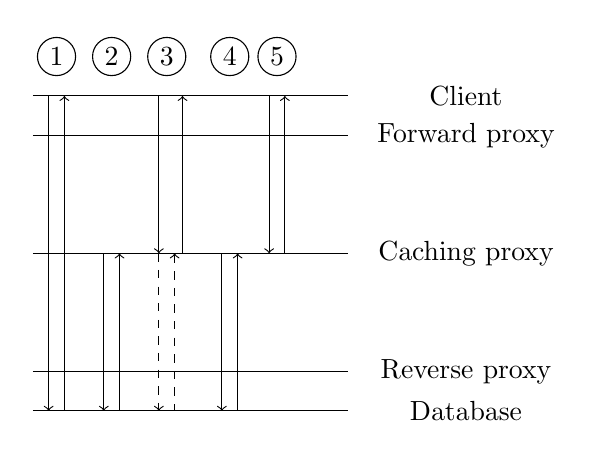
\begin{tikzpicture}
\draw (0,0) --(4,0);
\node at (5.5,0) { Database };
\draw (0,0.5) --(4,0.5);
\node at (5.5,0.5) { Reverse proxy };
\draw (0,2) --(4,2);
\node at (5.5,2) { Caching proxy };
\draw (0,3.5) --(4,3.5);
\node at (5.5,3.5) { Forward proxy };
\draw (0,4) --(4,4);
\node at (5.5,4) { Client };

\draw [->] (0.2,4) --(0.2,0);
\draw [<-] (0.4,4) --(0.4,0);
\node at (0.3,4.5) {\circled{1}};
\draw [->] (0.9,2) --(0.9,0);
\draw [<-] (1.1,2) --(1.1,0);
\node at (1.0,4.5) {\circled{2}};
\draw [->] (1.6,4) --(1.6,2);
\draw [dashed, ->] (1.6,2) --(1.6,0);
\draw [dashed, <-] (1.8,2) --(1.8,0);
\draw [->] (1.9,2) --(1.9,4);
\node at (1.7,4.5) {\circled{3}};
\draw [->] (2.4,2) --(2.4,0);
\draw [<-] (2.6,2) --(2.6,0);
\node at (2.5,4.5) {\circled{4}};
\draw [->] (3,4) --(3,2);
\draw [->] (3.2,2) --(3.2,4);
\node at (3.1,4.5) {\circled{5}};
\end{tikzpicture}
\caption{The possible positions of a cache. A cache may reside at both
  the server side (as a database cache) or client side, or any of the
  intermediate proxies. The arrows illustrate requests (when pointing
  down) and responses (when pointing up) in a deployment scenario for
  when the query cache considered in this paper is deployed on a
  caching proxy in the Internet infrastructure (see the text for
  details).}\label{fig:messaging}
\end{center}
\end{figure}

The system is based on HTTP, which implies a client-server
architecture. In this architecture, a cache may be present at
conceptually five different levels. First, the client may have its own
cache, which caches only responses made by the client itself. The next
level is known as a forward proxy. They aren't currently very common,
but have in the past often been institutional proxies, or proxies
employed by Internet Service Providers for caching responses that may
be common to many of their users. The next level, generically referred
to as a caching proxy, may be in the Internet
infrastructure. Currently, the most common form of this type of proxy
is known as a Content Delivery Network (CDN). It is very common to
have a reverse proxy near the server. They are often known as a ``Web
Accelerator''. Usually, they will communicate with the server with
HTTP, but it is conceivable that it may use a different protocol, and
may employ detailed knowledge of the hosted data to optimise cache
operations. Finally, the database, in this context a SPARQL Endpoint,
may use conventional database caching techniques. The database cache
and reverse proxy is typically controlled by the data provider.

The present system may be deployed at any of these levels (and similar
figures could be drawn). However,
since the database and the reverse proxy in front of it may have
detailed knowledge of the data, e.g. a complete data profile with
statistics to optimise join order, these levels have much in common
with a conventional database cache, which is extensively discussed in
the literature.

My interest is the case where the caching proxy has no further
knowledge of the data than what is exposed through the SPARQL Endpoint
or hypermedia metadata. While this would be known as a mediator in the
database literature and has also been a field of study for 20 years, I
focus on a practical motivation stemming mainly from what is currently
available. In current practice, very little information is available
to the mediator. Also, this study is also practically restricted to
HTTP. If the cache is to be shared, then it would typically reside on
the forward proxy, or in a CDN.

It is further interesting to note the contrast to the HERMES
\cite{adali1996query} system's concept of invariants discussed in
Section~\ref{sec:relcache}: a SPARQL query cache be oblivious
to domain knowledge in a CDN deployment and therefore shouldn't assume any invariants,
except in the possible but unlikely case where the remote server
declares an infinite freshness lifetime for the result of a certain
graph pattern. A forward proxy, on the other hand, may have a deeper
understanding on the needs of the client, and could possibly implement
invariants. The Attean framework accommodates for this.

Figure~\ref{fig:messaging} illustrates the case where HTTP messages
are being passed, where the cache is assumed to reside on a
intermediate caching proxy in the Internet, i.e. a CDN. The figure
may be viewed as having time on the $x$-axis, with the arrows pointing
down being requests and the arrows point up being responses. In this
example, the client first makes a request (request \circled{1}), which
is passed through the proxy because it has not yet cached any
responses. The response (response \circled{1}) is then also
transmitted directly from the SPARQL Endpoint at the database back to
the client. The entire response may be cached on the proxy in case it
can be reused in its entirety. However, the main point is that the
request will be analysed by the proxy in parallel to being sent to the
server, and another request \circled{2} for a triple pattern fragment
that the analyser thinks will enable the proxy to assist the server
the best for future requests, is sent. This analysis is discussed in
Section~\ref{sec:analpre}. The response \circled{2} is not sent back
to the client, but will enter the cache. Lets say that the analyser
was successful and that the cache can be used to answer request
\circled{3}. In that case, the proxy will send rewritten queries for
the rest of the data it needs to be able to answer the query to the
origin server, indicated by the dashed arrows. This may be zero or more SPARQL
query, TPF requests or a combination thereof, depending on what the
planner finds least expensive. The proxy will then evaluate the entire
query and send the final result back as response \circled{3}. In
addition, the analyser may have identified another Triple Pattern
Fragment that it takes as likely to be useful for future requests, and
sends a request and caches the response \circled{4}. At some point, it
may be able to answer the entire query using only cached results, as
illustrated by request and response \circled{5}.

Finally note that in this text, the term Triple Pattern Fragment (TPF)
is understood as a specialisation of Linked Data Fragments (LDF), in
which a Triple Pattern Fragment server must be able to answer any
triple pattern, whereas for a Linked Data Fragments server, this is
not required. However, there is no difference in the current
implementation, so in practice, the terms could be used
interchangeably.

\subsection{Key Problems}

\section{Implementation}\label{sec:impl}

The implementation consists of several modules that have been
published to the Comprehensive Perl Archive Network as Free Software,
and most of which have become a part the Free Software ecosystem. For
a detailed account of the modules that are a part of the system and
the authors that have contributed code in this ecosystem, see
Appendix~\ref{app:modules}.



\subsection{The Attean Framework}\label{sec:attean}

The Attean framework was born from the experiences the PerlRDF
community gained with \pmodule{RDF::Trine}, the Perl counterpart to
the more well-known Jena framework, and the opportunities presented by
the introduction of traits \cite{traits}, or roles as they are known
to the Perl world.

Traits are groups of methods that serve as a primitive unit of code
reuse. Traits are not constructed into objects themselves and do not
use inheritance for composition, instead a class is composed by a set
of traits and possibly the class' own methods, and then
instantiated. A trait can also require a set of methods or attributes,
and as such, is similar to an interface, but since its focus is code
reuse, it can also provide a default implementation.

The Attean framework packages commonly used classes when using
Semantic Web data, like RDF statements and terms, parsers,
serializers, triple/quad stores, iterators, but also features that are
relevant to query answering, like algebra, query planners and
plans. Additionally, it has an underlying extensive API consisting of
roles that can be composed to the above classes.

Perl is an interpreted language and is not focused on speed. Instead,
the focus is on developer efficiency. However, our motivation for
Attean, expressed in \cite{williamspushing}, was to enable the use
of faster implementations by using roles. It also serves to simplify 
code reuse.

For this work, the usage of roles to simplify query planning is of
particular importance. While we do not exploit optimisations closer to
the database, we extend the query planner in several directions with
several separate add-on modules, with only generic functionality in
the core Attean framework.

We have found it convenient to use classical inheritance in
combination with traits-based composition, but only when the base
class provide just fundamental functionality that is very likely to be
common to all implementations. For an example of this, see
Section~\ref{sec:implqueryplan}.

Also of importance are the APIs to compose stores. Stores in Attean
can be triplestores or quadstores, they can be mutable,
bulkupdateable, can enable the use of ETags or modification times for
conditional requests (as defined in RFC7232 \cite{rfc7234}), and makes
possible further extensions. Each of these primitives is represented
by a role that implements default functionality or simply requires
such functionality to be required. For instance, a quadstore is
required by \pmodule{Attean::API::QuadStore} to implement the
\pcode{get\_quads} method, which can take an RDF term as one or more
of the arguments and variables for the rest, and should return an
iterator over the quads that were matched. Based on an implementation
of the \pcode{get\_quads} method, the \pmodule{Attean::API::QuadStore}
role provides default implementations of methods \pcode{count\_quads},
\pcode{count\_quads\_estimate}, \pcode{get\_graphs} and
\pcode{size}. These methods may be overridden with more efficient
implementations when composing a class. Composing other roles will
require further methods to be implemented.

Stores can be rather diverse, so in addition, Attean provides another
abstraction layer, called a Model. Models consistently operate over
quads, in the case where underlying store is a triplestore, a graph
name will be set, or it may wrap several triplestores with a graph
name for each. In addition, Models provide higher level methods,
for example a \pcode{subject} method to list all subjects, and
corresponding for other terms. Thus, upper layers of an application
should use the Model abstraction. We have also chosen to implement significant
parts of the query planning in the Model.

When a query is parsed, algebra objects are generated. Based on the
algebra tree, models may generate plans for any algebra object of
their choosing by implementing the \pmodule{Attean::API::CostPlanner}
role. This amounts to implementing \pcode{plans\_for\_algebra} and
\pcode{cost\_for\_plan} methods. For a given algebra, Attean's query
planner will trust that the model's \pcode{plans\_for\_algebra} is
better than its own by default, a choice that was justified in
\cite{williamspushing}. Additionally, Attean has a simpler mechanism
for single quad patterns: By default, quad patterns are evaluated by
calling the Model's \pcode{get\_quads}, but this may be augmented by
adding a wrapper around an \pcode{access\_plans} method used by the
query planner to produce further plans.

Based on the algebra tree and plans generated by the models or the
default query planner, as well as the access plans, several
alternative plans will be generated, and their cost will be
estimated. How this happens in detail depends on how the planner is
composed. Attean comes with two roles that implement different
planners, \pmodule{Attean::API::SimpleCostPlanner} will compute all
possible plans and then estimate the cost of all plans, and finally
return the best 5. \pmodule{Attean::API::IDPJoinPlanner}
implements an Iterative Dynamic Programming planner
\cite{Kossmann:2000:IDP:352958.352982}, which prunes plans
aggressively based on their estimated cost in each iteration of query
plan generation. When a final plan tree has been found, the query may
be executed. 

That new plan types can be integrated into the planner with ease, and
that the planner itself can be changed with very little effort is a
key contribution of the Attean system, which I have taken advantage of
in this work. That this is made easy is to the credit of traits, as
will become clear as we study the details of the implementation in
Section~\ref{sec:implqueryplan}.


\subsection{SPARQL Protocol Client}\label{sec:sparqlclient}

The \pmodule{AtteanX::Store::SPARQL} module is a partial SPARQL
Protocol client that implements Attean APIs. The store implementation
itself composes the \mbox{TripleStore} API and implements methods to retrieve
the results of a single triple pattern and exact cardinality for a
given triple pattern, by using an aggregate query. In addition, it can
generate plans for Basic Graph Pattern algebra objects that have more
than one triple pattern. If that is the case, it will return an
instance of the class \pmodule{AtteanX::Plan::SPARQLBGP}, which is
also defined by the module. If it is not the case, the module also has
an implementation of the \pcode{access\_plan} method in a
\pmodule{AtteanX::Query::AccessPlan::SingleQuadBGP} role, that can be
composed by a query planner to provide a single triple pattern
\pmodule{AtteanX::Plan::SPARQLBGP} object. Finally, it also provides a
model implementation that composes the Model and \mbox{CostPlanner}
APIs. This contains a \pcode{cost\_for\_plan} implementation that will
provide a cost for \pmodule{AtteanX::Plan::SPARQLBGP} objects that are
proportional to the number of triple patterns in the plan, but
penalises plans that do not have triple patterns that are connected
through a variable (i.e. will cause a Cartesian join) with a factor
10. See Section~\ref{sec:costheuristics} for details on the cost
heuristics.

\subsection{Linked Data Fragment Client}\label{sec:ldfclient}

The Linked Data Fragment client work was started prior to this project
by Patrick Hochstenbach, and consists of the client code for Triple
Pattern Fragments in \pmodule{RDF::LDF}. It also includes the Basic
Graph Pattern optimisation from \cite{verborgh2014querying}. Included with the client
code is an implementation of a triplestore of the legacy
\pmodule{RDF::Trine} framework that predates Attean. He also started
an Attean store implementation \pmodule{AtteanX::Store::LDF} as a
separate module, but that module was subsequently adopted by me, and I
have written most of the functionality. It composes the \mbox{TripleStore}
and \mbox{CostPlanner} APIs and implements triple pattern queries and
cardinality estimates, both provided by the underlying client code as
they are a part of the core functionality of TPF,
as well as \pcode{cost\_for\_plan}.

It also supplies a plan class \pmodule{AtteanX::Plan::LDF::Triple}
used in the query planning. 

\subsection{The Caching Proxy}\label{sec:cacher}

The caching proxy consists of several components:

\begin{itemize}
\item Analysers, used to determine whether certain triple patterns
  should have their results prefetched and cached.
\item A prefetcher that performs the needed actions.
\item Two query planners, one that can use a local cache and a remote
  endpoint, and another that extends this to be able to use Triple
  Pattern Fragments as well, and corresponding models.
\item Two roles to generate plans for accessing cache and Triple
  Pattern Fragments and a corresponding plan class to enter results
  in the cache.
\item A custom User Agent for caching.
\item The actual caching proxy that accepts queries, runs the planner
  and returns the results.
\item Scripts to run the whole system.
\end{itemize}

In terms of technical contribution, most of these are
straightforward. The proxy itself, for example, is just a few lines of
wrapper code around the \pmodule{AtteanX::Endpoint} module. The User
Agent is a class that composes the roles of
\pmodule{LWP::UserAgent::CHICaching} and adds a hash of the query as
the cache key.

The main technical contributions are in the analysis of the query and
in the query planning.

\subsubsection{Analysis and Prefetching}\label{sec:analpre}

Analysers and prefetchers run asynchronously with query
evaluation. This is achieved by an addition to the proxy that sends a
query to a persistent analyser script that subscribes to a channel on
a Redis\footnote{See \url{http://redis.io/}} data structure store. 

The analyser script can be configured to use any number of analysers.
Two such analysers have been implemented, for now constrained to
single triple patterns. One will count the predicates in consecutive
queries it sees, and publish triple patterns to another Redis channel
with the predicate if the count exceeds a certain configurable
limit. This is an attempt to capture and cache popular parts of
queries.

The second analyser will rerun the query planner on the incoming query
while simulating that the results of a certain triple pattern was in
the cache. If the cost reduction of the best plan is larger than a
configurable limit, it will publish that triple pattern to the same
Redis channel as above. 

Another persistent script is subscribed to this latter channel. If the
Model supports LDF, a retriever will then download
the results of the triple pattern and enter it into the cache, or use
a single triple pattern SPARQL query if not. The current
implementation assumes that both and LDF server and a SPARQL endpoint
can be used to answer any triple pattern. Relaxing this assumption
depends on that the LDF specifications gain stronger semantics to link
SPARQL endpoints and LDF servers together. With that, the assumption
could be abandoned trivially.

The cache itself is assumed to only cache the results of triple
patterns where at least one term is bound. 
I have used the Redis data structure store for the
cache as well. This choice is somewhat arbitrary, and has not proved
very successful. The cache will store the results as an array if two
RDF terms are bound in the triple pattern, or a hash if only one term
is bound. The strings put into the cache are serialized N-Triples
strings.

In addition to caching the prefetched results, the proxy may also
cache the serialized results of any full SPARQL query, and also enter
the results of any Linked Data Fragment retrieved when the query
planner evaluates a query into the above cache, using a trivial
extension to the plan class in Section~\ref{sec:ldfclient}.



\subsubsection{Query Planner}\label{sec:implqueryplan}

The query planner is written as completely stand-alone modules, based
on the facilities in the Attean framework, but without accessing
Attean internals. The system has in fact three query planners:
\pmodule{AtteanX::QueryPlanner::Cache},
\pmodule{AtteanX::QueryPlanner::Cache::LDF} and
\pmodule{AtteanX::Query::Cache::Analyzer::QueryPlanner}. Each is an
extension of the previous. The first is written to use a remote
endpoint in combination with a local cache. The second extends this to
also be able to generate and use TPF plans. The
final is a query planner for the analyser in Section~\ref{sec:analpre}
that reruns the query planning with all triple patterns in a simulated
cache.

These query planners are a good example of the virtues of traits-based
programming, as they are typically customised along different axes:
access plans, cost estimation, planning of joins within Basic Graph
Patterns or left joins, rewriting (like gathering quad patterns to
blocks), etc. In the case of our query planner that combines a remote
endpoint with a local cache, named
\pmodule{AtteanX::QueryPlanner::Cache}, the basic query planner of the
Attean framework, \pmodule{Attean::QueryPlanner} is extended
(i.e. inherited from), but also composes the following roles:
\pmodule{Attean::API::NaiveJoinPlanner},
\pmodule{Attean::API::SimpleCostPlanner},
\pmodule{AtteanX::API::JoinRotatingPlanner},
\pmodule{AtteanX::Query::AccessPlan::SingleQuadBGP} and
\pmodule{AtteanX::Query::AccessPlan::Cache}, out of which the three
first are a part of the Attean framework, the next was described in
Section~\ref{sec:sparqlclient} and the last is a part of the
query cache system itself.


\pmodule{Attean::QueryPlanner} has only minimal functionality,
everything else is provided by the roles. Conventional single
inheritance is constrained to a tree structure, and would result in a
very complex system. Another option is to use the factory method
pattern, where a factory object would need to be initialised to return
a suitable object for each axis of customisation. 

It is interesting to detail the function of
\pmodule{AtteanX::API::JoinRotatingPlanner}. Its main function is to
produce alternatives for join query plans. For example, if we have
three quad patterns $A$, $B$ and $C$, plans for both $ ( A \bowtie B)
\bowtie C $ and $ A \bowtie ( B \bowtie C ) $ will be generated. In
some cases, it may be possible to reduce a join to a more fundamental
plan type, and this may be done next. In our case, this is done in
\pmodule{AtteanX::QueryPlanner::Cache}, where adjacent quad patterns
are coalesced into Basic Graph Pattern (BGP) plans, and BGP plans are
coalesced into larger BGP plans, so that they can be evaluated by the
remote SPARQL endpoint as a single unit. This will minimise the number
of HTTP requests, in much the same way as the exclusive groups of
\cite{springerlink:10.1007/978-3-642-25073-6-38}. Note, however, that
the generated plans are subject to cost estimation, so whether a large
BGP plan will be evaluated remotely, or as a join of local cached
results and a smaller remote BGP, or in the case of
\pmodule{AtteanX::QueryPlanner::Cache::LDF}, a remote Triple Pattern
Fragments server, is up to the cost estimation. This will be discussed
in detail in Section~\ref{sec:costheuristics}.

\subsection{Cost Model}\label{sec:costheuristics}

The final query execution is designed to be entirely cost-based,
i.e. many alternative plans are generated, but the decision on whether
to use a certain plan is entirely up to the cost model. While the
framework is flexible and could support further research into cost
models, I have considered this to be future work, and only a small
heuristic cost model is present in the current system. 

However, since the combination of remotely executed SPARQL with a
local cache and TPF is rather complex, the cost
heuristics are fairly elaborate. Moreover, since the objective of the
study is to take load off of the remote endpoint, the heuristics are
intended to make the proxy work harder than the remote endpoint.

Throughout the system, the query planner takes the cost from the
models implementing the \pmodule{Attean::API::CostPlanner} role. A
key challenge is to balance the costs given by different models in the
system, and this is done in
\pmodule{AtteanX::Model::SPARQLCache::LDF}. Let us, however, start
from the bottom. 

The cost of evaluating a Triple Pattern Fragment plan $C_{tpf}$ is estimated to
be 
\begin{equation}
C_{tpf} = 10 + \floor{990 \frac{n_{tpf}}{n_{tot}}} ,
\end{equation}
where $n_{tpf}$ is the estimated number of triples expected to be
matched by the triple pattern and $n_{tot}$ is the size of the
model. Thus, this cost will be an integer between 10 and 1000. The
reason we use a floor function is that the Attean cost model only
supports integers.

The cost of accessing the cache is assumed to be small compared to the
above, and is estimated as 
\begin{equation}
C_c = 2 + \floor{\log_{10}{n_c}} , 
\end{equation}
where $n_c$ is the number of triples in the cache that matches the
given triple pattern.

The cost of evaluating a remote SPARQL query is estimated to be the
number of subplans (usually quad patterns) incremented by one and
multiplied by 100 if there is a common variable between all the
subplans, or 1000 if there is not. This is to prevent the remote
endpoint from having to compute Cartesian joins as much as possible. A
remote SPARQL query with only one triple pattern is assumed to always
be more expensive than to evaluate than a Triple Pattern Fragment
(recall that we want to relieve the remote endpoint of stress), and so
is given the cost of 1001.


Next, we detail the cost of a join where one or more children in the
tree is a remote SPARQL plan. It is usually not wanted to execute
several remote queries, it is assumed that the number of HTTP requests
should be small, and that plans where the joins have been rotated and
coalesced by \pmodule{AtteanX::API::JoinRotatingPlanner} should be
less expensive. Therefore, such plans should be penalised, but by how
much depends on the type plans. Conventionally, for a nested loop join
plan, we multiply the cost of the subplans, increment the resulting
cost by one if the right hand plan is more expensive than the left
hand plan, and multiply by a factor of 10 if there are no shared
variables, to mildly penalise Cartesian joins. If the plan is a hash
join the difference is that, we add rather than multiply the cost of
the of the subplans, and multiply by a factor of 100 rather than 10 so
that if it is necessary to evaluate a Cartesian join, it is more
likely done using a nested loop join. Then, the resulting cost is
multiplied by the number of remote SPARQL Basic Graph Patterns in the
tree and the factor 1.2, and floored to the nearest integer.

Under the assumption that it is better to join remotely than to
possibly retrieve large amounts of data, a similar algorithm is used
to penalise join plans that contain many Triple Pattern Fragment
plans, by multiplying the cost of the join plan by the number of the
Triple Pattern Fragment plans in the tree.

Finally, if a plan has a Triple Pattern Fragment plan that has a
common variable with a remote SPARQL query, that plan is given an
added cost to 1000, to allow plans where the triple pattern has been
rotated into the BGP win, again to reduce the amount of data needed to
be transferred.

\section{Evaluation}

The system was developed in a practically oriented test-driven manner,
with emphasis on testing cases that I assumed \textit{a priori} to be
difficult. The interested reader may like to refer to the published code,
given in Section~\ref{sec:impl}. Some of the tests consist of a number
of queries, and some of the tests concern the problem I found in a
preliminary study, that the cached triples would often break
subsequent queries to cause Cartesian joins. Much of the above cost
model is designed to prevent this from having a detrimental impact.

While I am quite confident that the code is producing query plans as
intended and that analysis and prefetching is able to retrieve and
cache results, an elaborate evaluation would be needed to explore
further whether the system actually helps remote endpoints and is able
to serve clients with adequate performance. Unfortunately, the
evaluation showed that the latter is not the case with the current
implementation, and the practical constraints of the project then
prevented further investigation. Thus, this section consists of an
account of the evaluation that was performed and the methodology I
planned to employ.

\subsection{Actual Evaluation}

I decided to set the entire system up as a proxy server, and run a
realistic query against DBpedia repeatedly. The intention was to let
the analyser find all required data and eventually add that to the
cache. Once the cache was filled with all the data, the query cache
should be able to answer the query on its own, at least within a time
period on the order of a magnitude of the original endpoint (which
took on the order of 1~second). 

The following query was used:

\begin{verbatim}
PREFIX foaf: <http://xmlns.com/foaf/0.1/>
PREFIX dbo: <http://dbpedia.org/ontology/>
SELECT ?name WHERE {
  ?s a foaf:Person ;
     foaf:name ?name ;
     dbo:wikiPageID  9828878 .
} ORDER BY ?name
\end{verbatim}

The query was chosen because of its wide variety in terms of
selectivity of the individual triple patterns. The retriever managed
to pull all the data from the LDF version of DBpedia
within some hours. 

The cache was kept in a Redis data structure database on a machine
with a Intel Core2 Duo E8500 CPU with 16 GB of RAM. The proxy server
with the query engine ran on a Intel Xeon CPU E3-1230 v5 CPU with 32
GB of RAM, residing a LAN with a gigabit Ethernet link between
them. Running the query on this hardware took more than 1000 seconds
without any performance analysis enabled. This is clearly more than
two orders of magnitude longer than acceptable. Moreover, it is then
clearly not possible to draw any conclusions as to whether the system
would be helpful in achieving its goal of taking load off of the
remote server, as it could process far fewer queries than the public
remote endpoint, and any load saved on the remote endpoint would
likely be less than the uncertainty arising from that.

Nevertheless, it is interesting to further understand this failure. In
Table~\ref{tab:nytprof}, I have tabulated the result of the subroutine
calls that take the most time.

\begin{table}
\caption{Top 15 Subroutines Calls as measured by the profiler \pmodule{Devel::NYTProf}.}\label{tab:nytprof}

\begin{tabular}{r p{1.5cm} p{1.5cm} l}
  \hline
Calls & 	Exclusive Time & Inclusive Time & Subroutine \\
\hline
13309080	& 244s	& 549s & \pcode{IRI::\_parse\_components} \\
13309080	& 218s	& 218s & \pcode{IRI::CORE:match (opcode)} \\
8774329	        & 116s	& 270s & \pcode{Attean::Result::new} \\
10573035	& 111s	& 1420s & \pcode{AtteanX::Parser::NTuples::\_eat\_node} \\
6355072	 	& 79.7s & 1856s & \pcode{Attean::CodeIterator::next} \\
2 & 77.4s & 4540s & \pcode{Attean::Plan::HashJoin::\_\_ANON\_\_[Attean/Plan.pm:362]} \\
4217970		& 70.0s & 847s & \pcode{Attean::Literal::new} \\
9091102	 	& 61.8s	& 593s & \pcode{Attean::IRI::new} \\
2419260	        & 50.3s & 208s & \pcode{Attean::API::Result::join} \\
4217968	        & 48.7s	& 1463s & \pcode{AtteanX::Query::AccessPlan::Cache::\_\_ANON\_\_[AtteanX/Query/AccessPlan/Cache.pm:72]} \\
24186545	& 48.1s	& 56.6s & \pcode{Role::Tiny::does\_role} \\
28128408	& 44.4s	& 53.8s	& \pcode{Attean::Result::value} \\
16871877	& 44.1s	& 470s & \pcode{Attean::Literal::\_\_ANON\_\_[(eval 234)[Class/Method/Modifiers.pm:93]:1] (merge of 4 subs)}\\
4217969		& 40.0s & 92.0s & \pcode{Attean::API::Literal::\_\_ANON\_\_[Attean/API/Term.pm:160]} \\
13309111	& 39.5s & 39.5s & \pcode{IRI::CORE:regcomp (opcode)}
\end{tabular}
\end{table}

It is clear that the vast majority of time spent is due to my cache
implementation. When using the Redis cache, I serialise RDF terms as
N-Triples, and when they are retrieved, they have to be parsed and
instantiated as objects for the query engine. Remarkably, parsing of
Internationalized Resource Identifiers (IRIs) is the single most
time-consuming task. While each parse does not take much time, it
happens more than 13~million times. The reason why parsing IRIs
happens is that a certain amount of parsing is required to compare
them \cite{rfc3987}, and the \pmodule{IRI} module is a rigorous
implementation of the standard that does syntax based resolution if
the if an object is constructed with a base. IRI parsing happens not
only when an \pmodule{Attean::IRI} object is constructed, but may also
happen when an \pmodule{Attean::Literal} object is constructed, since
the data type is a IRI.

While most of the time is spent in parsing and comparison, the hash
joins also require too much time. A discussion of possible
improvements will follow in Section~\ref{sec:discussfail}.

\subsection{Planned Evaluation}\label{sec:planned}

This section outlines the evaluation I had planned to employ on the
query cacher. The essence is to perform a ``query log replay, while
recording remote endpoint load under different circumstances,
determined by a experiment designed with statistical Design of
Experiments formalism''. 

In more detail, query logs can be obtained from
for example USEWOD~\cite{eps385344} or the Linked SPARQL Queries
Dataset \cite{Saleem2015}. An extraction of one of those datasets
could be performed, to create a representative progression of
queries. The data normally residing on a remote endpoint
(i.e. ``server'') would then be loaded into a single database system
under my control. A proxy system would be set up using our
system. Finally, a client would submit the queries to the server, via
the proxy. 

On the server, some metric of system load would be recorded. In
statistical experimentation parlance, this is known as the ``response
variable''. I had not entirely decided which metric to use, but
\cite{Ferrari:1987:EIL:647412.725013} indicated the load average may
be a good choice. It could be trivially recorded by polling the
virtual file \texttt{/proc/loadavg} on the host system. Possibly a
correction for any extra time spent by the proxy could be applied.

As for the overall design of the experiment, the reader may refer to
the paper discussed in Section~\ref{sec:condoe} for an introduction to
the type of evaluation intended to be used. As noted, a $2^n$
factorial experiment is the simplest experiment to set up, and I would
therefore go to great lengths to ensure that such an experiment could
be used.

It would also be advantageous to design the experiment so that a
combination of factors would correspond to the null hypothesis,
i.e. that the proxy was not in use and the remote endpoint would
tackle the whole load. I did not think this complete through to a
concrete experiment, but it might be a challenging problem to maintain
orthogonality, i.e. ensure that all level combinations can occur in
the same number of runs.

However, the factors that may be interesting to investigate include
both factors that evaluate the analyser and the query planner. These
factors might be:

\begin{enumerate}
\item Use of the cache and remote endpoints where the levels are on
  and off.
\item Use of a caching LDF client, levels on and
  off.
\item Use the predicate count analyser, levels on and off.
\item Use the best cost improvement analyser, levels on and off.
\item The order of the application of the different methods for
  analysis.
\item Which cost planner to use, with levels being the simple cost
  planner and the Iterative Dynamic Programming planner, see
  Section~\ref{sec:attean}.
\end{enumerate}

While this design would achieve the goal that a combination of levels
would correspond to the null hypothesis, certain levels are somewhat
problematic. For example, the LDF client in point~2
might be an implementation of \cite{verborgh2014querying}, but that
would be very different from the combination of point~1~and~2, which
correspond to the usage of
\pmodule{AtteanX::QueryPlanner::Cache::LDF}. Additionally, I noted
that downloading the triple pattern fragment
\sparql{?s~foaf:name~?name~.}  
resulted in more than 40~000 HTTP requests due to
paging. Another relevant factor might be to deploy a Triple Pattern
Fragments server that does not page, and have levels with paging on
and off. Integrating this factor in the experimental design would
further complicate it.

If the experiment outlined here could come to fruition, and we take
the factor in the first point with level~1 as the cache being enabled,
then we can examine the experiment similarly to what with did with the
``Implement'' factor in \cite{kjernsmo_doe_intro}. That is, the first
step to understand the contributions to the endpoint system load by
the different factors, is to create a normal plot and then use the
Lenth criterion for significance. For the next step, to test the
alternative hypothesis that the endpoint system load has decreased,
form an average of the effects for all combinations of the factor in
point~1 and the insignificant factors determined in the first step,
based on the average over the rest of the factors. Based on this, a
common one-sided two-sample $t$-test can be performed.\todo{Discuss
  cost model based on DoE?}


\section{Discussion}

\subsection{Join Rotation and Iterative Dynamic
  Programming}

While the system used a simple brute-force query planner in the above
evaluation, using an Iterative Dynamic Programming planner
\cite{Kossmann:2000:IDP:352958.352982} would simply amount to
composing \pmodule{Attean::API::IDPJoinPlanner} in the planner class.

While this performed better in most cases, the test suite contains a
query where it does not:
\begin{verbatim}
?s <http://example.org/m/p> "1" ;
   <http://example.org/m/p> ?o ;
   <http://example.org/m/q> _:xyz ;
   <http://example.org/m/q> <http://example.org/m/a> .
?a <http://example.org/m/b> <http://example.org/m/c> .
\end{verbatim}
Note that the above Basic Graph Pattern contains a triple pattern that
does not share a variable (\sparql{?a}) with any other triple pattern,
thus creating a problematic Cartesian join. Additionally, in this
test, the results of the two first triple patterns have been
cached. \textit{A priori}, I have assumed that the best plan is a plan
where the cache is used for these two triple patterns, the last triple
pattern is answered by a LDF server and the last two
triple patterns are coalesced into a new SPARQL query, and evaluated
remotely. This is also coded as a pass criterion for the test. With
the simple query planner, this test passes, but not with the IDP
planner, as it results in a plan where the two triple patterns that
should run is a single SPARQL query are split into two. This resulted
in an interesting observation:

As noted in Section~\ref{sec:implqueryplan}, we rely on rotating joins
to gather triple pattern plans into a larger structure that can be
evaluated together, like a remote SPARQL BGP. On careful inspection, I
found that the join rotation would have had to descend into
great-grandchildren of the top join plan. However, with the IDP
planner, plans are aggressively pruned, and therefore, this
constellation is not considered. This led us (with Gregory Todd
Williams) to conjecture that this weakness is inherit to IDP planning
(and possibly a general problem with any early-pruning planner) 
when using join rotation. However, we did not attempt to examine this any
further.

To remedy this problem, we considered creating a custom query planner
for Basic Graph Patterns, but this was not implemented. The outline
would have been as follows:
\begin{enumerate}
\item Find triple patterns that are connected with a common variable,
  and group them to ``components''.
\item If a triple pattern has a cached result, create a plan that
  accesses the cache. 
\item If the triple pattern in the previous step causes a Cartesian
  join to be created within a component, create an equivalent
  additional plan for a SPARQL remote evaluation that does not access
  the local cache.
\item Any remaining components consisting of a single triple pattern
  result in LDF plans.
\item Any remaining components are turned into SPARQL remote BGP
  plans.
\end{enumerate}

This procedure would allow the cost model to balance the cost between
doing a Cartesian join and doing a remote SPARQL evaluation of data
already in the cache, as plans for both these options would be
provided.\todo{Discuss algebra equivalences here?}

\subsection{Remedies for Performance Issues}\label{sec:discussfail}

The issue could be raised that it was a bad idea to begin with to use a
scripting language like Perl to write a query engine with performance
requirements. Indeed, that may be the case. However, generally
accepted practice is to first find the actual performance issues and
then optimise using a bridge to first and foremost the C family of
languages as needed. Importantly, with the width of the scope, I only
had some months to implement the query engine. This is not a software
engineering project, but given past industrial experience, it seems
unlikely that I could have achieved it within the allowed time frame
using older paradigms, such as the factory method pattern.

The profiling points out a clearly where large gains could be
made. First and foremost, parsing must be avoided, and that could be
avoided by ensuring that IRIs where canonicalised before they were
written to the cache, so that comparing them later would be a simple
string comparison. Secondly, the Redis data structure store could be
better exploited to store strings that could be used to construct  
literals and IRI objects without parsing. 

However, since computing the join itself is too slow, it is not
necessarily a solution worth pursuing. The main motivation behind
caching hashes and arrays in Redis was to save space; since at least
one term would be bound in any cached pattern, it shouldn't be
necessary to insert more data into the cache. Since the performance of
doing the join is poor, this may not be justified. Instead, it may be
a better idea to use a conventional quad store for the cache. In that
case, the planner would require a simple modification so that triple
patterns are gathered into locally evaluated BGPs and remotely
evaluated BGPs as well as LDFs. To take full advantage of this
approach, SPARQL 1.1 \sparql{VALUES} would also need to be supported,
so that the local quad store could perform all join operations. With
this in mind, I wrote a rudimentary Virtuoso store driver for Attean, but
at that point, the project was overdue and needed to be concluded. 

It seems likely that the project, with more time, could be brought to
the point where the evaluation in Section~\ref{sec:planned} could be
applied, and new insight could be gained.

Thus, the main contribution from this project is the ease
with which it was implemented.

\begin{subappendices}
%\renewcommand{\setthesection}{\Alph{section}}
%\renewcommand{\setthesubsection}{\Alph{subsection}}


%\section{Appendix}
\section{Appendix: Modules and Their Contributors}\label{app:modules}


To
install the system on the top of a Debian system with only essential
packages requires 146 Debian packages. Running the test suite requires
even more. As such, it builds on the code of hundreds of authors, too
many to enumerate. I shall constrain myself to list the modules that
have code that has been motivated by this study. Modules that have
other primary authors than myself have been started prior to this
present project, but may have substantial contributions from this
project. The Attean framework was started as part of the effort in
Section~\ref{sec:conpush}, but even though it has been developed
further with the requirements that arose from this project and has
contributions from me, the vast majority of the code has been written
by Gregory Todd Williams. The main work in this project has gone into
the module \pmodule{AtteanX::Query::Cache}, where I have authored the
vast majority of the code. The relative difference in authorship can
be further examined by checking the linked Github repositories, or by
using git2prov\footnote{See \url{http://git2prov.org/}} to create RDF
data of the commit history. Table~\ref{tab:modules} shows the modules
that have been influenced or written as part of this project.

\begin{table}
\caption{The modules that enable the query cache}\label{tab:modules}
\begin{tabular}{ | l | p{3cm} | l |}
  \hline
  Module & Authors & Github URL \\ \hline

  \pmodule{AtteanX::Query::Cache} & Kjetil Kjernsmo, Gregory Todd Williams &
  \url{kjetilk/p5-atteanx-query-cache} \\ % 0.001_04

  \pmodule{AtteanX::Store::SPARQL} & Kjetil Kjernsmo &
  \url{kjetilk/p5-atteanx-store-sparql} \\ % 0.008
  
  \pmodule{AtteanX::Store::LDF} & Kjetil Kjernsmo, Patrick Hochstenbach &
  \url{phochste/AtteanX-Store-LDF} \\ % 0.02

  \pmodule{LWP::UserAgent::CHICaching} & Kjetil Kjernsmo &
  \url{kjetilk/p5-lwp-useragent-chicaching} \\ % 0.04
  
  \pmodule{Attean} & Gregory Todd Williams, Kjetil Kjernsmo &
  \url{kasei/attean} \\ % 0.015

  \pmodule{AtteanX::Endpoint} & Gregory Todd Williams &
  \url{kasei/atteanx-endpoint} \\ % 0.001

  \pmodule{RDF::LDF} &  Patrick Hochstenbach, Gregory Todd Williams, Jakob Voß,
  Kjetil Kjernsmo & \url{phochste/RDF-LDF} \\ % 0.17
  
  \hline
\end{tabular}
\end{table}
\todo{make it fit. Rotate?}

The system also depends on modules I have written that are not part of
the project: \pmodule{RDF::LinkedData}, \pmodule{RDF::Generator::Void}, \pmodule{Test::RDF},
\pmodule{URI::NamespaceMap} and \pmodule{RDF::NS::Curated}.

To further understand the roles of the different modules, note the
following: \pmodule{LWP::UserAgent::CHICaching} is a traits-based
\cite{traits} implementation of the majority of RFC7234.
The underlying caching framework used by this module, \pmodule{CHI},
will take care of expiry and purging of entries, since this module
will supply an explicit freshness lifetime. 
\pmodule{AtteanX::Endpoint} is an implementation of the server side of
SPARQL 1.1 Protocol. 

\end{subappendices}


%%  LocalWords:  canonicalised


\bibliography{management,dataprofiles,federation,dynamicity,hypermedia,specs,webarch,practical,semweb,caching,critisism,data,philosophy,benchmarks,rfc,programming,egne,optimization}
\bibliographystyle{plain}

\chapter{Papers}

The following papers are used for this thesis:
\begin{itemize}
\item Kjetil Kjernsmo.
\newblock The Necessity of Hypermedia RDF and an Approach to Achieve it.
\newblock In {\em Proceedings of the First Linked APIs workshop at the Ninth
  Extended Semantic Web Conference}, May 2012.
\item Kjetil Kjernsmo and John~S. Tyssedal.
\newblock Introducing Statistical Design of Experiments to SPARQL Endpoint
  Evaluation.
\newblock In Harith Alani, Lalana Kagal, Achille Fokoue, Paul Groth, Chris
  Biemann, Josiane~Xavier Parreira, Lora Aroyo, Natasha Noy, Chris Welty, and
  Krzysztof Janowicz, editors, {\em The Semantic Web – ISWC 2013}, volume
  8219 of {\em Lecture Notes in Computer Science}, pages 360--375. Springer
  Berlin Heidelberg, 2013.
\item Gregory~Todd Williams and Kjetil Kjernsmo.
\newblock Pushing Complexity Down the Stack.
\newblock In {\em Proceedings of the ISWC Developers Workshop 2014}, volume
  1268 of {\em {CEUR} Workshop Proceedings}. CEUR-WS.org, May 2014.
\item Kjetil Kjernsmo.
\newblock A Survey of HTTP Caching Implementations on the Open Semantic Web.
\newblock In Fabien Gandon, Marta Sabou, Harald Sack, Claudia d’Amato,
  Philippe Cudré-Mauroux, and Antoine Zimmermann, editors, {\em The Semantic
  Web. Latest Advances and New Domains}, volume 9088 of {\em Lecture Notes in
  Computer Science}, pages 286--301. Springer International
  Publishing, 2015.
\item Kjetil Kjernsmo.
\newblock Addendum to a survey of {HTTP} caching on the {Semantic Web}.
\newblock Technical Report 444, Department of Informatics, University of Oslo,
  March 2015.
\item Kjetil Kjernsmo and Ruben Verborgh.
\newblock How can scientific methods provide guidance for semantic web research
  and development.
\newblock In {\em Workshop on Negative or Inconclusive Results in Semantic Web
  Proceedings}, volume 1435 of {\em {CEUR} Workshop Proceedings}. CEUR-WS.org,
  2015.
\end{itemize}



\includepdf[pages=1-last,openright,scale=1.2]{/home/kjetil/uio/www_docs/2012/hypermedia-rdf.pdf}
\includepdf[pages=1-last,openright,scale=1.2]{/home/kjetil/uio/www_docs/2013/iswc.pdf}
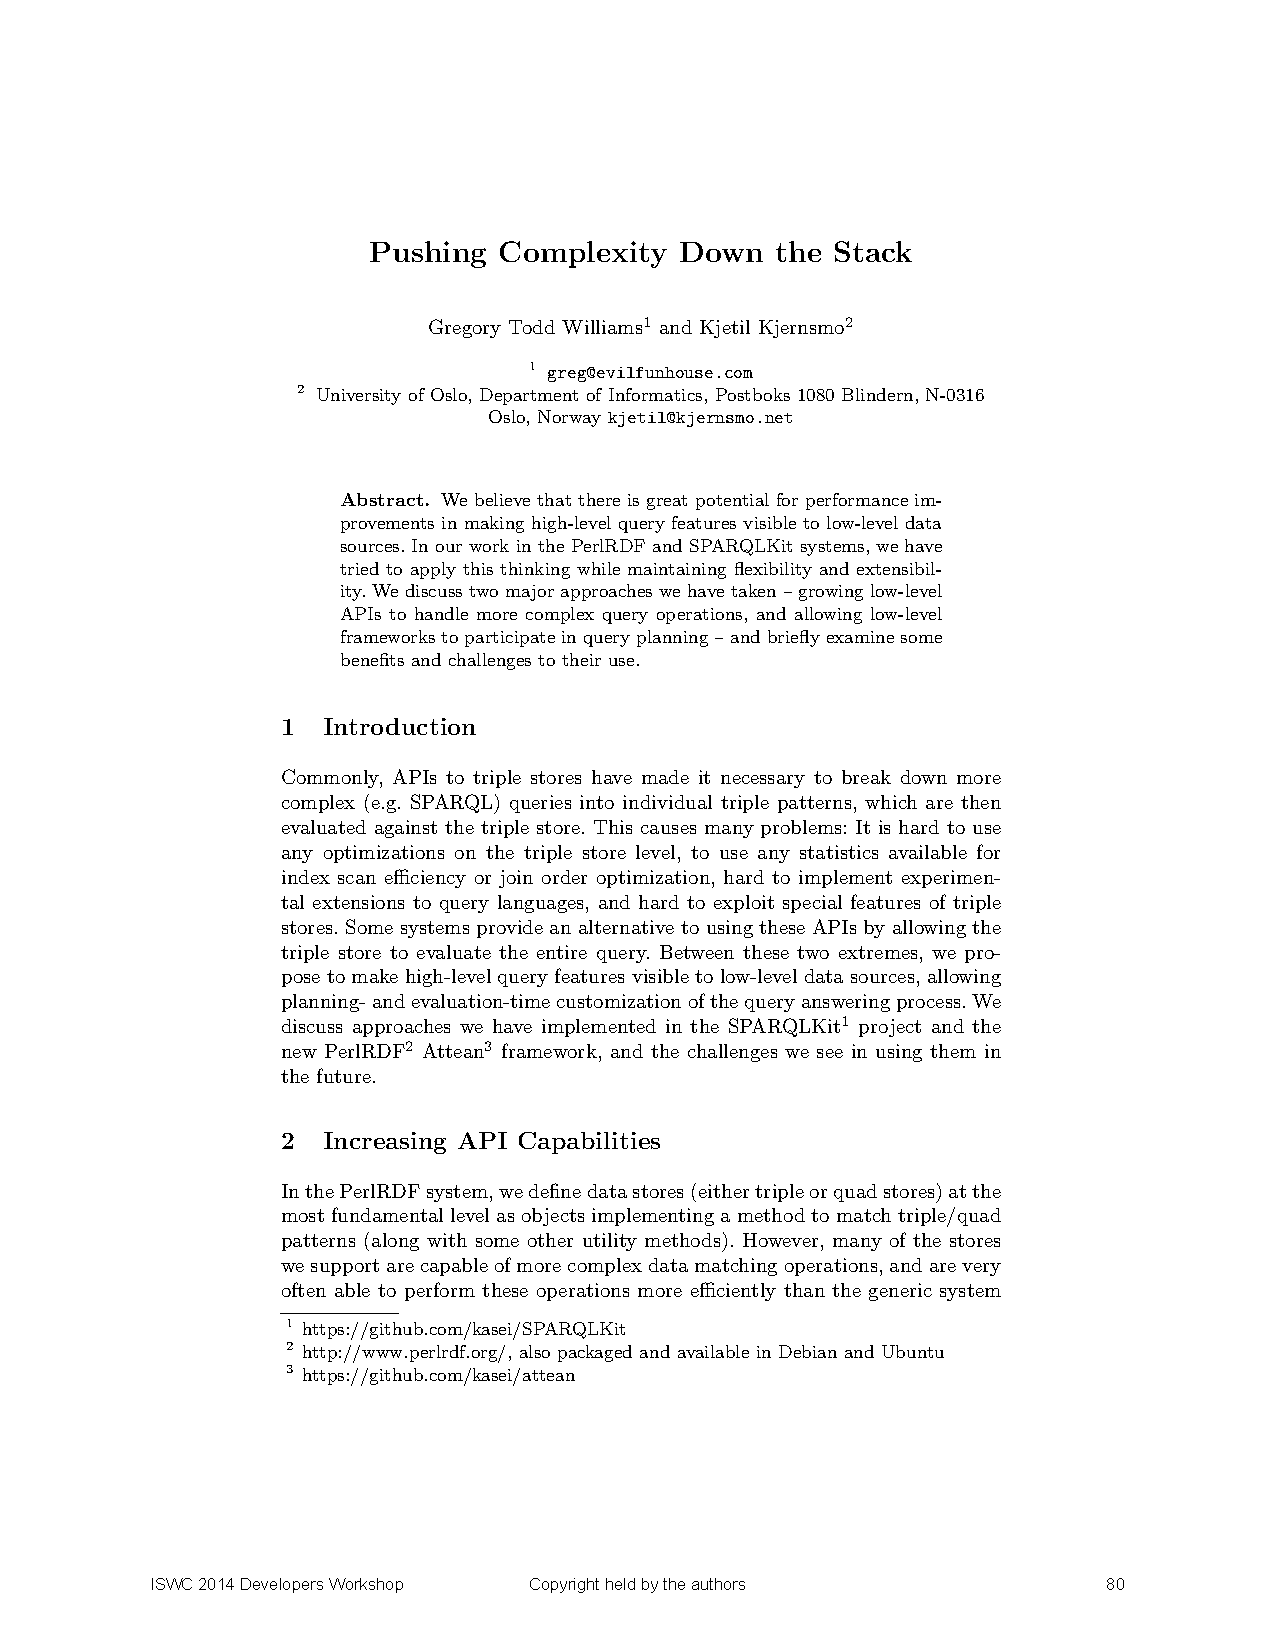
\includepdf[pages=1-last,openright,scale=1.2]{paper14.pdf}
\includepdf[pages=1-last,openright,scale=1.2]{/home/kjetil/uio/www_docs/2015/cache-survey.pdf}
\includepdf[pages=1-last,openright]{report.pdf}
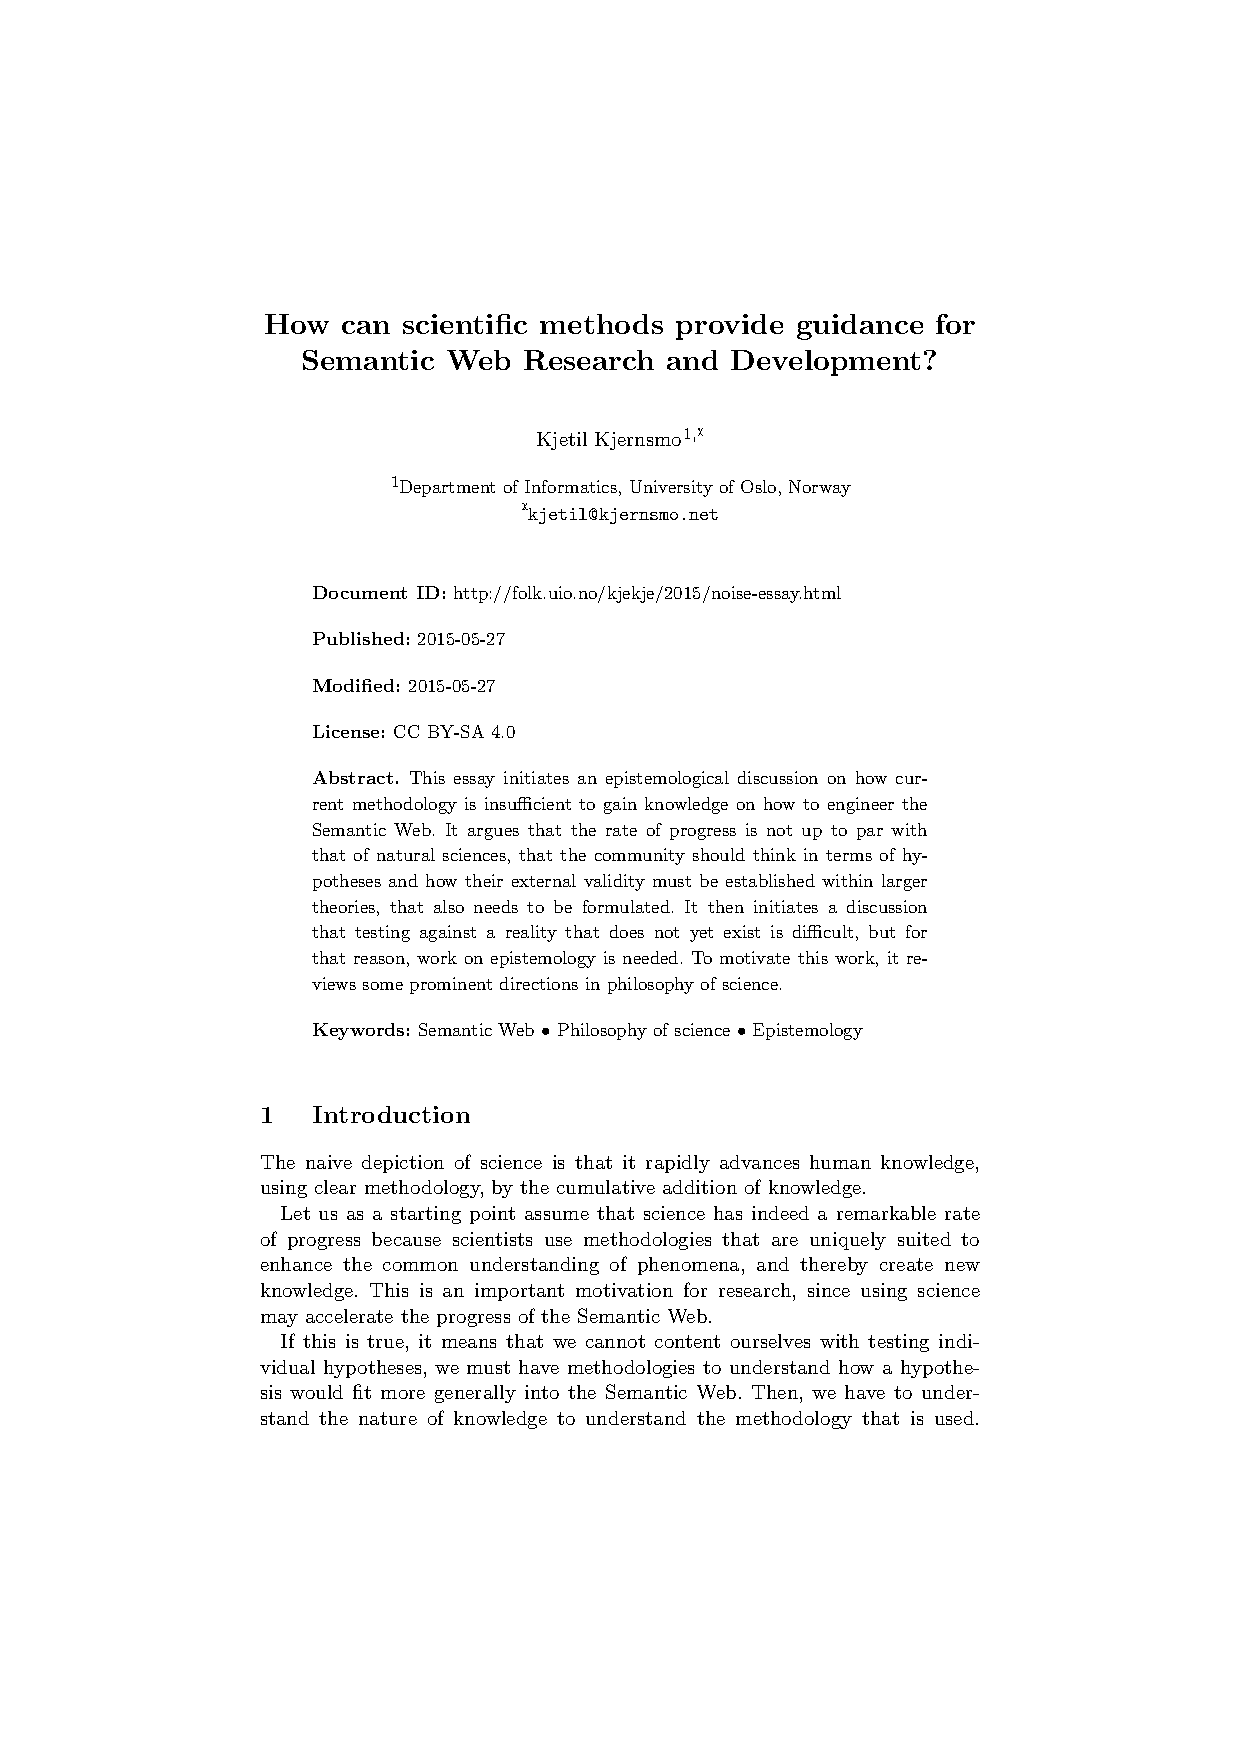
\includepdf[pages=1-last,openright,scale=1.2]{noise.pdf}
\end{document}
